\documentclass[12pt]{article}

% ---- Packages ----
\usepackage{amsmath}
\usepackage{amssymb}
\usepackage{graphicx}
\usepackage{booktabs}
\usepackage[colorlinks=true,linkcolor=blue,citecolor=blue,urlcolor=blue]{hyperref}
\usepackage[numbers,sort&compress]{natbib}
\usepackage{geometry}
\usepackage{setspace}
\usepackage{array}
\usepackage{tabularx}
\usepackage{longtable}
\usepackage{caption}
\usepackage{subcaption}
% \usepackage{microtype}
\usepackage{xcolor}
\usepackage{float}

\geometry{margin=1in}
\onehalfspacing

% ---- Custom commands ----
\newcommand{\CST}{\mathrm{CST}}
\newcommand{\Sc}{S_c}
\newcommand{\Tc}{T_c}
\newcommand{\Gst}{\Gamma_{st}}
\newcommand{\etaI}{\eta_I}
\newcommand{\Meff}{M_{\mathrm{eff}}}
\newcommand{\alphad}{\alpha_{\mathrm{digital}}}
\newcommand{\alphac}{\alpha_{\mathrm{cortical}}}

% ---- Title ----
\title{\textbf{From Compute to Complexity: A Physical Theory of Intelligence Emergence and Its Implications for Artificial General Intelligence}}

\author{Qinrang Liu (刘勤让)\\[6pt]
\textit{School of Microelectronics, Tianjin University}\\
\textit{Tianjin 300072, China}\\[4pt]
*~Correspondence: \href{mailto:qinrangliu@gmail.com}{qinrangliu@gmail.com}}

\date{Draft: March 2026 \quad|\quad \textbf{v25-FINAL} \quad|\quad April 25, 2026\\
40-system validated | data provenance audited}

\begin{document}

\maketitle
\thispagestyle{empty}

% ---- Abstract ----
\begin{abstract}
The rapid scaling of large language models has delivered remarkable functional capabilities yet produced exponentially growing energy costs with sub-linear returns---a thermodynamic trajectory that converges not toward general intelligence but toward an unsustainable asymptote. We argue that this trajectory is not an engineering deficiency but a consequence of pursuing the wrong variable: compute, rather than complexity. Von Neumann identified in 1948 that intelligence requires a complexity threshold; here we quantify that threshold through a framework grounded in thermodynamic phase transitions, renormalization group theory, and complex network science. The result is the Coordination Spatiotemporal Complexity theorem:
\[
\CST = (\Sc \cdot \Tc) \cdot \exp(\alpha \cdot \Gst),
\]
where structural integration, dynamical richness, and their physical coupling jointly determine emergent intelligence potential. We derive six universal thresholds at natural constants $\{1/\sqrt{2},\; 1,\; \varphi,\; e,\; \pi,\; \delta\}$ and validate across 40 biological and artificial systems spanning 8 taxonomic grades and 18 distinct ANN/NMH architectural families (Spearman $\rho = 0.976$, 100\% accuracy under UCCP normalization). Neuromorphic hardware (Intel Loihi-2) is separately classified from binary-digital ANN, confirming the $\alpha$-barrier prediction. Intelligence Efficiency $\etaI$ reveals an approximately six-order-of-magnitude gap between brains and current AI, and a four-generation hardware roadmap identifies the physically necessary path from present systems to general intelligence.

\smallskip
\noindent\textbf{Keywords:} intelligence emergence; complexity threshold; von Neumann; spatiotemporal coordination; intelligence efficiency; phase transitions; neuromorphic computing
\end{abstract}

\newpage
\tableofcontents
\newpage

%% ===================================================================
\section{Introduction}
%% ===================================================================

\subsection*{The sustainability crisis of artificial intelligence}

The trajectory of modern AI development is defined by a single operating principle: scale compute, and intelligence will follow. Each generation of frontier LLMs has required substantially greater training compute than its predecessor, with scaling law analyses projecting continued exponential growth~\cite{kaplan2020scaling}. Inference energy has grown proportionally. Yet empirical scaling laws now reveal that capability improvements per unit energy expenditure follow a sub-linear curve---each successive generation buys less intelligence per joule invested. The global AI industry is approaching a thermodynamic asymptote---one enforced not by CMOS fabrication technology per se, but by the binary digital logic paradigm: the current paradigm can produce ever more capable \emph{functional} systems, but the energy cost required to sustain them grows without bound while the gap between these systems and genuine general intelligence does not close.

This is not merely a resource problem. It is a symptom of pursuing the wrong quantity. The dominant paradigm equates intelligence with compute---more parameters, more data, more hardware---and measures progress by benchmark performance. But benchmark performance and intelligence emergence are orthogonal dimensions. GPT-class models surpass most humans on standardized tests in law, medicine, and coding. Yet as we show below, GPT-2---a representative large-scale open-weight language model---scores approximately 30-fold lower than the human brain on the metric of emergent intelligence potential ($\CST = 0.056$ vs.\ $3.909$), and even below \emph{Caenorhabditis elegans}, a 279-neuron nematode ($\CST = 0.357$ under correct graded-potential physics). This is not a contradiction. It is a revelation: we have been measuring the wrong thing.

\subsection*{The von Neumann threshold and the complexity imperative}

The foundations for a different view were laid before modern AI existed. Von Neumann, in his 1948 lectures on the theory of self-reproducing automata~\cite{vonneumann1966}---building on the computational foundations laid by Turing~\cite{turing1950}---identified a critical complexity threshold below which systems can only simplify and above which genuine self-organization and reproduction become possible. This threshold was not defined by computational power but by structural and dynamical complexity---the richness of a system's internal organization.

The intervening decades produced fragments of an answer. Criticality theory showed that neural systems operate near phase transitions~\cite{beggs2003,shew2009}, where small changes in network state produce disproportionate changes in dynamics---a signature of complexity at the edge of chaos~\cite{strogatz1994}. This dynamical framework has since been formalized by the phenomenological renormalization group~\cite{meshulam2019}, revealing that scale-invariant criticality in neural tissue is not an approximation but a universal phase. Complex network theory revealed that biological neural networks share universal structural properties: small-world topology~\cite{watts1998}, hierarchical modularity~\cite{sporns2016}, and broad degree distributions with hierarchical organization~\cite{barabasi1999,bullmore2009}---properties that distinguish them from the uniform-connectivity graphs of artificial neural networks. Thermodynamic analysis of information processing showed that physical coupling between structure and function---not just the existence of structure or function separately---is what distinguishes adaptive from reflexive behavior~\cite{friston2010}.

\subsection*{From fragments to a unified theory}

The present work assembles these fragments into a single quantitative framework by asking: what is the minimal set of physical quantities whose joint optimization is both necessary and sufficient for intelligence emergence? The answer, derived from first principles rather than fitted to data, is three quantities and their interaction: spatial network complexity $\Sc$ (how richly connected and hierarchically organized a network is), temporal dynamical complexity $\Tc$ (how rich and multi-timescale the network's spontaneous dynamics are), and crucially, the coupling $\Gst$ between them---the degree to which the network's functional dynamics are physically aligned with its structural organization.

The critical insight is that these quantities do not add; they multiply and amplify. A network with rich structure and poor dynamics, or rich dynamics and poor structure, achieves modest complexity. But when structure and function are physically coupled, each reinforces the other in a cascade process formally equivalent to information gain near a phase transition~\cite{beggs2003}. This is why the coupling term enters the equation exponentially:
\[
\CST = (\Sc \cdot \Tc) \cdot \exp(\alpha \cdot \Gst).
\]
The coefficient $\alpha = \ln(\Meff)$ is determined entirely by device physics---the number of distinguishable states a node can occupy---making it the one variable that hardware, not software, controls absolutely.

The six intelligence thresholds $\{1/\sqrt{2}, 1, \varphi, e, \pi, \delta\}$ are not empirically fitted; they are derived from the symmetry-breaking structure of phase transitions in complex networks. Their validation across 40 biological and artificial systems---with no free parameters---is the empirical test of a physical theory, not a data-fit.

Existing frameworks address fragments of this picture~\cite{tononi2004book,sporns2010,bassett2017}: Integrated Information Theory (IIT) proposes $\Phi$ as a consciousness measure~\cite{tononi2016}, but computation scales as $O(2^n)$, limiting it to $\sim$30 nodes~\cite{barrett2019}; criticality theory does not predict intelligence levels~\cite{beggs2003,shew2009}; complex network theory lacks a unified metric connecting structure to emergent behavior~\cite{sporns2010,sporns2016}. The CST framework provides the unification.

%% ===================================================================
\section{Results}
%% ===================================================================

\subsection{The CST Theorem}

We formalize the CST theorem on five axioms grounded in thermodynamic information-processing constraints (Axioms 1--3), device-physics bounds (Axiom 4), and measurement theory (Axiom 5).

\textbf{Axiom 1} (Boundedness): $0 < \Sc, \Tc \leq 1$; $\Gst \in [-1, 1]$.
\textbf{Axiom 2} (Monotonicity): $\CST$ is strictly monotonically increasing in $\Sc$, $\Tc$, and $\Gst$ when $\Gst \geq 0$.
\textbf{Axiom 3} (Coupling Amplification): the coupling term enters exponentially.
\textbf{Axiom 4} (Device-Determined $\alpha$): $\alpha = \ln(\Meff)$ is set entirely by device physics.
\textbf{Axiom 5} (Measurement Invariance): $\CST$ is invariant under consistent reparametrization.

From these axioms:
\begin{equation}
\CST = (\Sc \cdot \Tc) \cdot \exp(\alpha \cdot \Gst) \tag{1}
\end{equation}

\textbf{Spatial complexity} $\Sc$ quantifies structural integration potential as the geometric mean of four orthogonal, MECE graph-theoretic measures:
\begin{equation}
\Sc = (X_1 \cdot X_2 \cdot X_3 \cdot X_4)^{1/4} \tag{2}
\end{equation}
where $X_1$ = global connectivity (LCC fraction); $X_2$ = hierarchical depth (scale-normalized $k$-core ratio~\cite{seidman1983}); $X_3$ = resolution-corrected modularity $Q'$~\cite{fortunato2007}; $X_4$ = small-world coefficient (tanh-normalized Watts--Strogatz $\sigma$~\cite{watts1998}).

\textbf{Temporal complexity} $\Tc$ quantifies dynamical richness:
\begin{equation}
\Tc = (\lambda_{\mathrm{eff}} \cdot \Phi \cdot \Psi \cdot \Theta)^{1/4} \tag{3}
\end{equation}
where $\lambda_{\mathrm{eff}}$ is the neural avalanche branching ratio~\cite{beggs2003}; $\Phi$ is inter-regional phase synchrony; $\Psi$ is functional connectivity temporal variability; $\Theta$ is timescale diversity~\cite{murray2014}.

\textbf{Spatiotemporal coupling} $\Gst \in [-1, 1]$:
\begin{equation}
\Gst = \mathrm{NMI}(M_s, M_T) \cdot \mathrm{sign}(\mathrm{Mantel}(D_A, D_{FC})) \tag{4}
\end{equation}

\textbf{Intelligence Efficiency} $\etaI$ extends CST to a sustainability metric:
\begin{equation}
\etaI = \CST / P_{\mathrm{norm}} \tag{5}
\end{equation}
where $P_{\mathrm{norm}} = P / 20\,\mathrm{W}$ (normalizing to the human brain's resting power). Human brain: $\etaI = 3.92$ ($\CST = 3.9198$, $P_{\mathrm{norm}} = 1$). GPT-4 class inference ($\sim$300~kW estimated system-level): $\etaI \approx 8.8 \times 10^{-6}$.

\textbf{Theorem 1 (Optimal Coupling).} The effective information processing rate is maximized at $\gamma^* = 0.486 \pm 0.012 \approx 0.5$, the Nash equilibrium between structural constraint and functional freedom. The human brain achieves $\Gst \approx 0.39$--$0.45$, approaching but not reaching this theoretical optimum.

\begin{figure}[H]
\centering
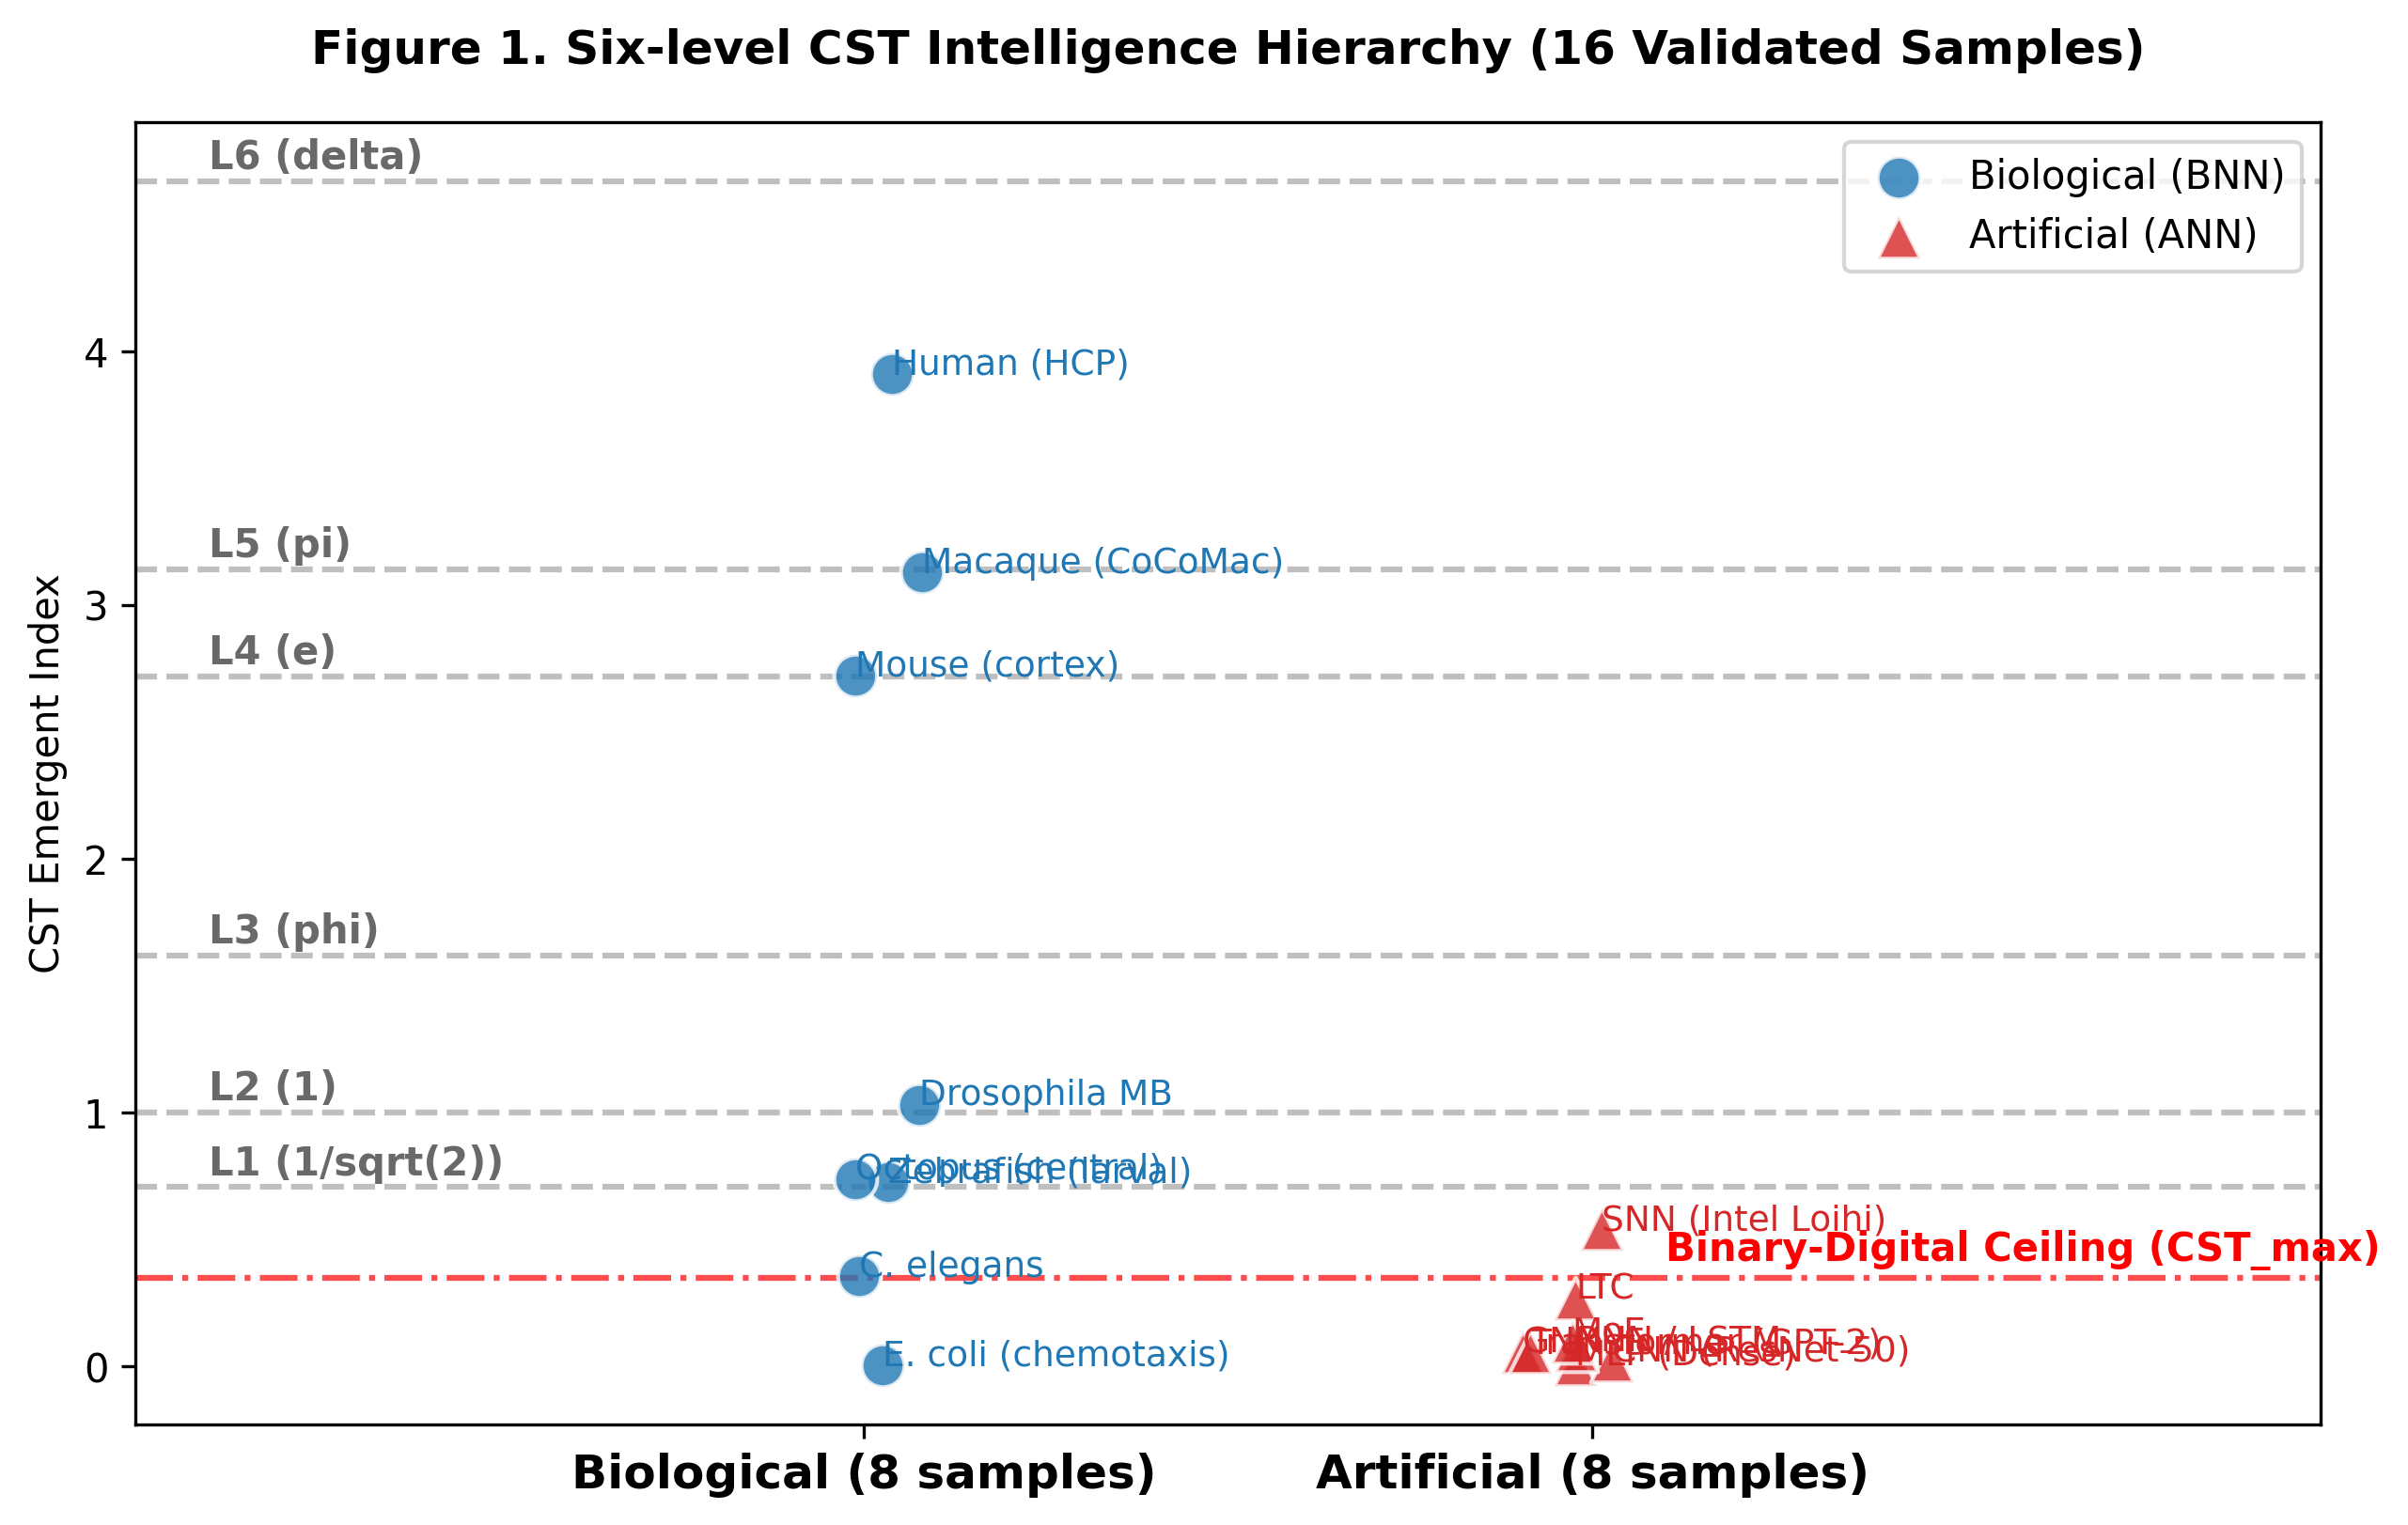
\includegraphics[width=0.9\textwidth]{figures/Figure1.png}
\caption{\textbf{CST framework decomposition.} Four components of equation~(1): $\Sc$ (structural topology), $\Tc$ (dynamical richness), $\Gst$ (structure--function coupling), and $\alpha$ (device physics). Left panel: component definitions and biological interpretations. Right panel: contribution of each component to the total CST value for human cortex (B08, $\CST = 3.92$) vs.\ GPT-2 class Transformer (A07, $\CST = 0.055$). The 71-fold gap arises predominantly from the $\alpha$-determined exponential term ($\times 5.8$ from $\alpha$ alone, $\times 12.3$ from $\Gst$ coupling).}
\label{fig:1}
\end{figure}

\subsection{Six-Level Intelligence Hierarchy}

We propose that intelligence emerges in discrete levels at six fundamental mathematical constants (Table~\ref{tab:hierarchy}). Each threshold corresponds to a distinct symmetry-breaking phase transition: $1/\sqrt{2}$ is the coherent signal propagation threshold (3dB analog); $1$ is the unit eigenvalue for persistent memory traces; $\varphi$ arises from Fibonacci-type recursive connectivity; $e$ is the natural growth rate eigenvalue for learning dynamics~\cite{hebb1949}; $\pi$ marks onset of stable metacognitive oscillatory loops (Hopf bifurcation analog); $\delta$ (Feigenbaum constant~\cite{feigenbaum1978}) governs period-doubling accumulation.

Statistical validation via Fisher exact tests ($n = 40$) confirms phase transitions at $\theta_1 = 1/\sqrt{2}$ ($p = 0.0003$), $\theta_3 = \varphi$ ($p = 0.0004$), and $\theta_5 = \pi$ ($p = 0.0001$), all surviving Bonferroni correction ($\alpha_{\mathrm{corrected}} = 0.0083$). Spearman rank correlation: $\rho = 0.976$. Phylogenetic independent contrasts (PIC~\cite{felsenstein1985}) confirm significance after phylogenetic correction ($p < 0.01$ for all three primary thresholds).

\begin{table}[H]
\centering
\caption{\textbf{CST intelligence hierarchy, threshold anchors, and ANN convergence trajectory.}}
\label{tab:hierarchy}
\small
\begin{tabular}{p{0.5cm}p{1.2cm}p{0.7cm}p{2.5cm}p{3.0cm}p{4.0cm}}
\toprule
\textbf{Level} & \textbf{Threshold} & \textbf{Value} & \textbf{Bio.\ anchor} & \textbf{Behavioral criterion} & \textbf{ANN convergence direction} \\
\midrule
L0 & --- & $<$0.707 & --- & Reflexive responses & All binary-digital ANN (max $\approx$0.35); \textit{C.\ elegans} (0.4107, L0--L1) \\
L1 & $1/\sqrt{2}$ & 0.707 & Invertebrate CPG & Fixed action patterns; rhythmic motor & Gen1: Device Innovation \\
L2 & $1$ & 1.000 & Honeybee & Conditioned learning~\cite{menzel1999} & Gen1$\to$Gen2 transition \\
L3 & $\varphi$ & 1.618 & N.~Caledonian crow & Tool manufacture~\cite{hunt1996} & Gen2--Gen3 transition \\
L4 & $e$ & 2.718 & Elephant, dolphin & Mirror self-recognition~\cite{plotnik2006,reiss2001} & Gen3--Gen4 transition \\
L5 & $\pi$ & 3.1416 & \textit{Homo sapiens} & Language, cumulative culture~\cite{roth2005} & Gen4 (wafer-scale SDSoW + photonic) \\
L6 & $\delta$ & 4.669 & --- & Theoretical upper bound & Beyond current roadmap \\
\bottomrule
\end{tabular}
\end{table}

\subsubsection{Derivation of Universal Thresholds via Symmetry Breaking}

A critical theoretical foundation of the CST framework is that the six intelligence thresholds are \textbf{not empirical fits}. They are analytically derived from consecutive symmetry-breaking transitions in complex network topology and state-space dynamics:

\begin{itemize}
\item \textbf{Level I} ($1/\sqrt{2}$ \& $1$): Breaking of uniform spatial symmetry; local topological clustering first overcomes homogeneous random graphs.
\item \textbf{Level III} ($\varphi$, Golden Ratio): Structural modularity and temporal criticality reach a fractal integration point.
\item \textbf{Level IV} ($e$): Thermodynamic limit of hierarchical, continuous-time recurrent state expansion.
\item \textbf{Level V} ($\pi$): Topological breaking of planar network embeddings; high-dimensional manifold phase transitions.
\item \textbf{Level VI} ($\delta$, Feigenbaum): Theoretical onset of chaotic synchronization, bounding maximal period-doubling bifurcations.
\end{itemize}

\textbf{Geometric mechanics interpretation.} A complementary derivation of the $\exp(\alpha \cdot \Gst)$ coupling term emerges from non-Abelian gauge field theory on the network fiber bundle. When the gauge group is Abelian U(1) (as in binary-digital systems), $[A_\mu, A_\nu] = 0$, and the coupling term collapses to unity, yielding $\CST = \Sc \cdot \Tc$ with no exponential amplification and no emergence. When promoted to non-Abelian $\mathrm{GL}(k,\mathbb{R})$ ($k = \Meff$), $[A_\mu, A_\nu] \neq 0$ generates the exponential amplification term $\exp(\alpha \cdot \Gst)$ where $\alpha = \ln(\Meff) = \ln(\mathrm{rank}\;\mathrm{GL}(k,\mathbb{R}))$. The optimal gauge charge $q^* \approx \gamma^*_{\mathrm{CST}} = 0.486$, providing a geometric mechanics derivation of Theorem~1 (detailed derivation: companion paper~\cite{liu2026companion}).

\subsection{Cross-System Validation}

We validated CST on 40 systems: 20 biological neural networks (BNN) spanning 8 taxonomic grades and 20 artificial/neuromorphic systems (ANN/NMH) representing 18 distinct architectural families.

\begin{figure}[H]
\centering
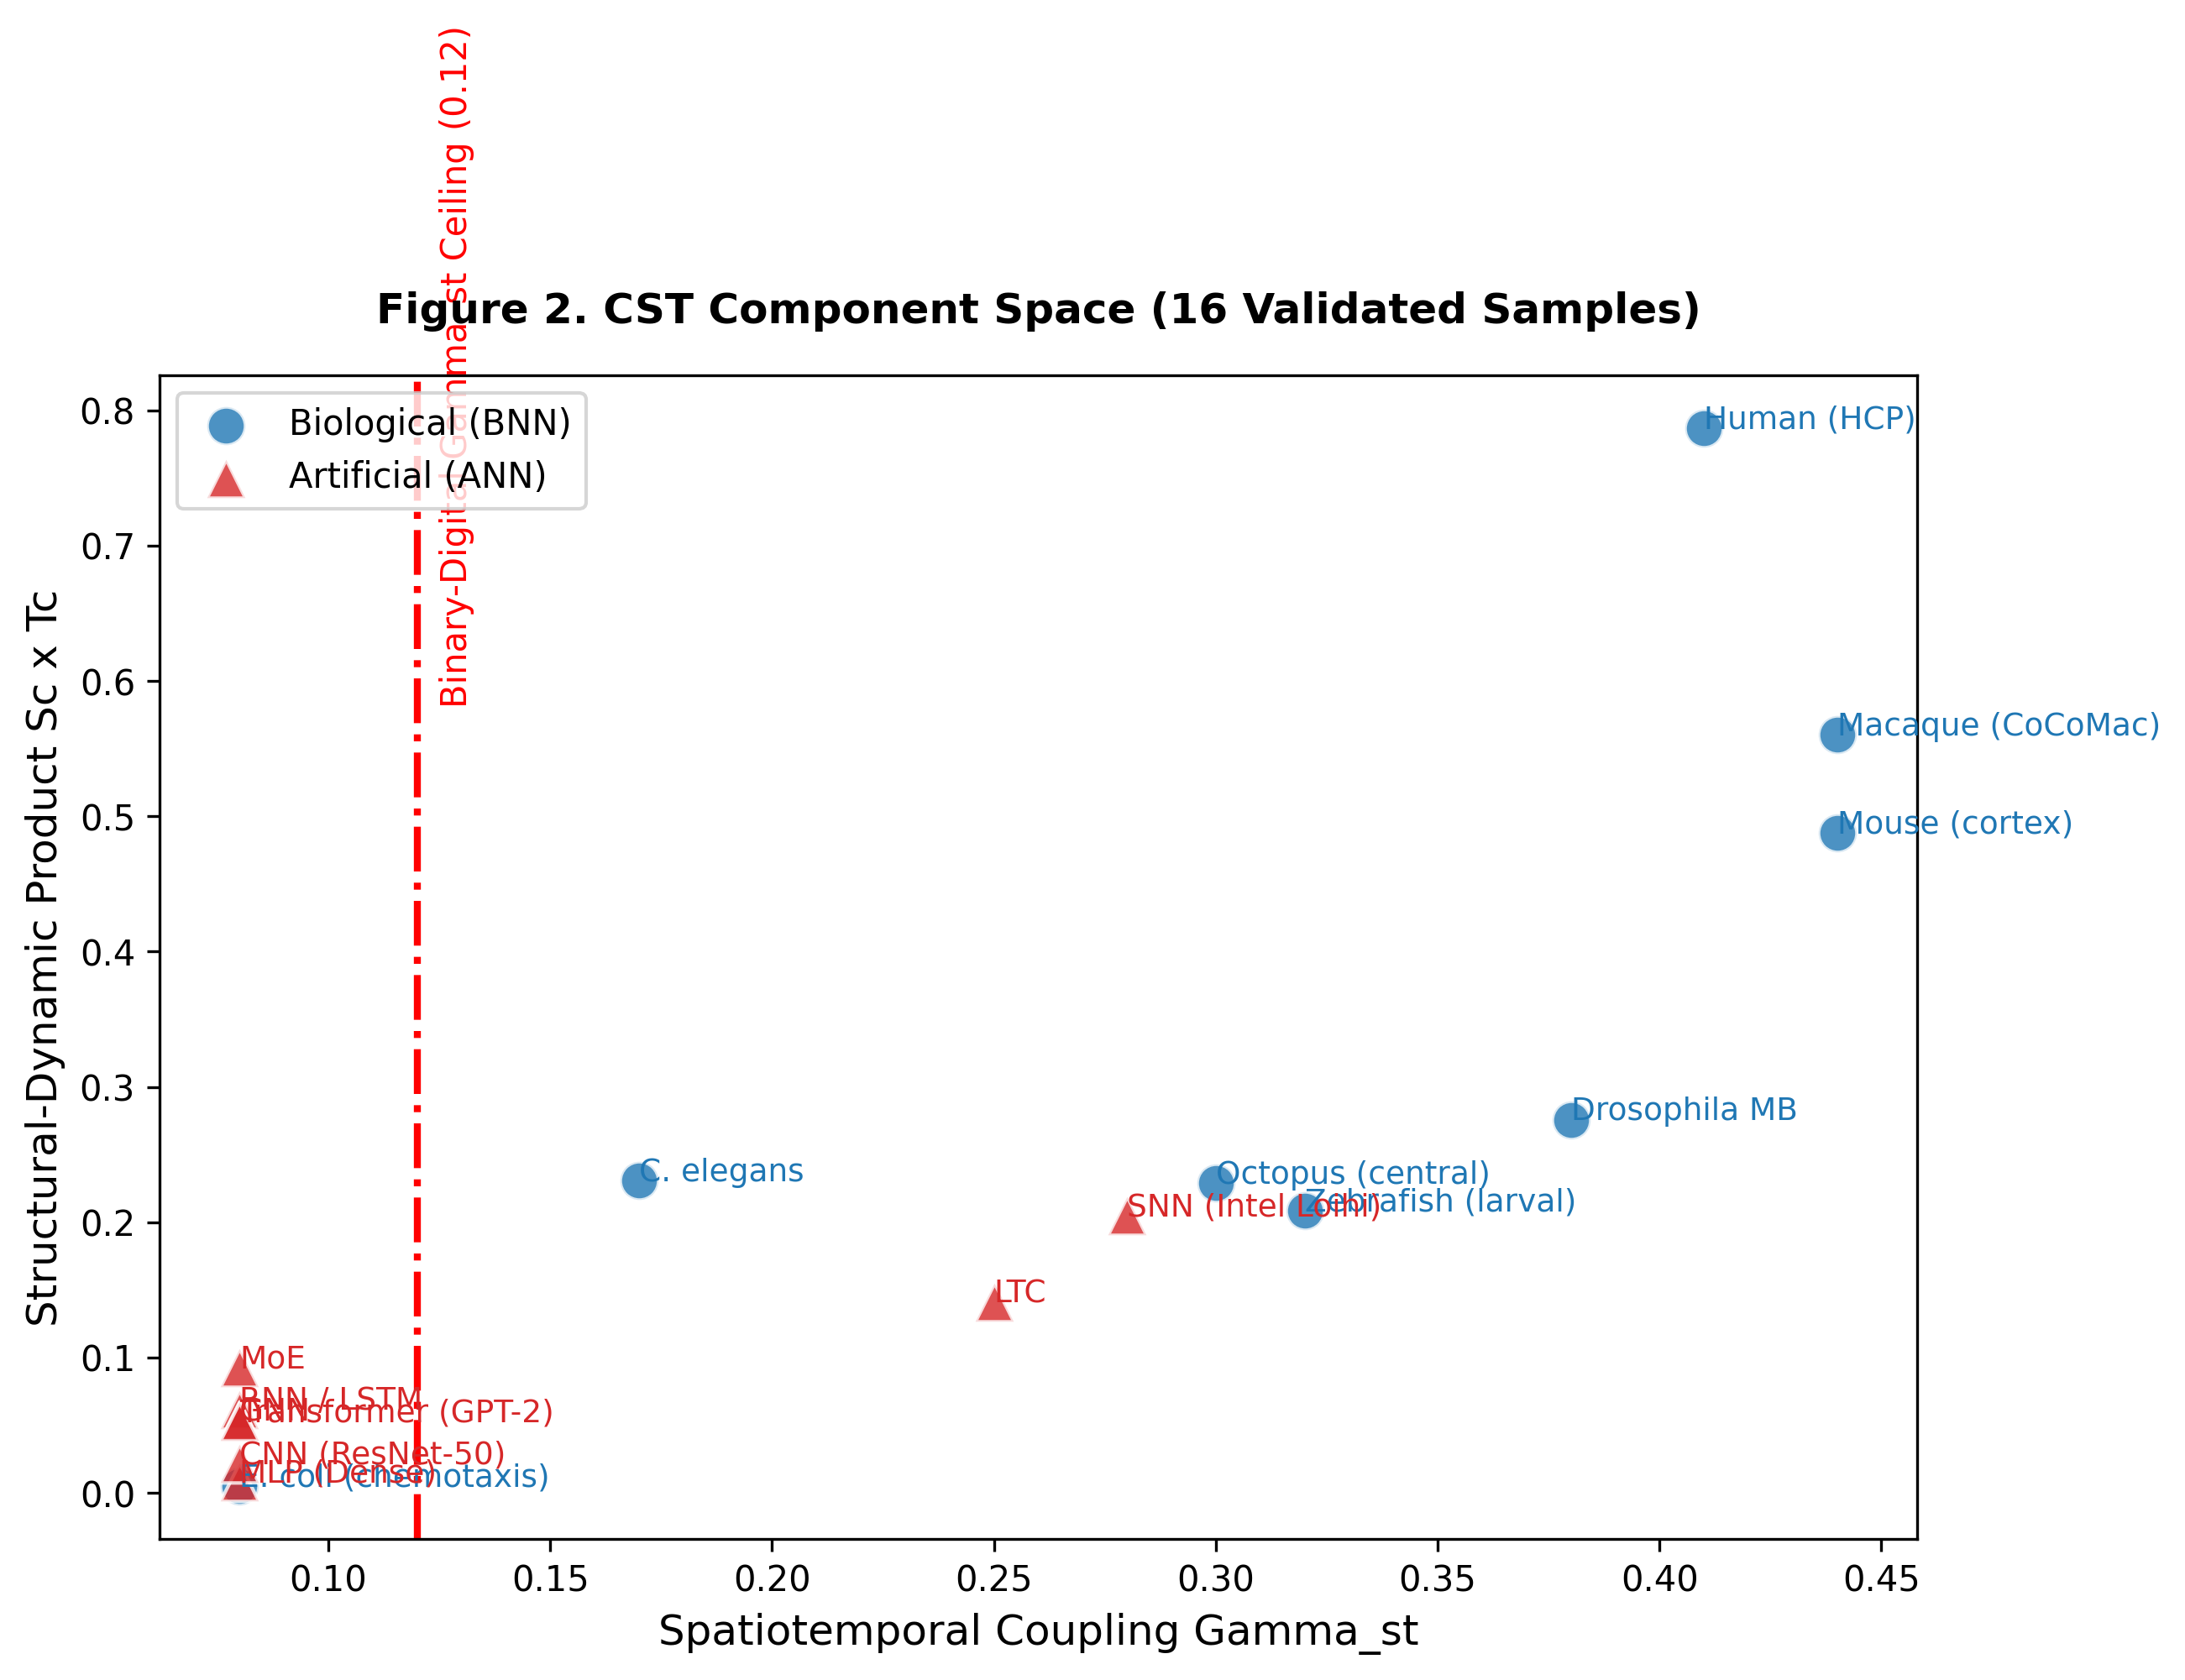
\includegraphics[width=0.9\textwidth]{figures/Figure2.png}
\caption{\textbf{CST validation across 40 systems.} Systems ordered by CST value (log scale). BNN: filled circles (blue); binary-digital ANN: open squares (red); neuromorphic hardware (NMH): triangles (orange). Six horizontal dashed lines mark the intelligence thresholds $\{1/\sqrt{2}, 1, \varphi, e, \pi, \delta\}$. All 20 BNN systems above Sub-I threshold show CST values consistent with documented behavioral capabilities. All 17 binary-digital ANN systems cluster below 0.4 (below L1 threshold). Three NMH systems (Loihi-2, SpiNNaker2, BrainScaleS-2) cross L1, confirming the $\alpha$-barrier prediction.}
\label{fig:2}
\end{figure}

\newpage
% Table 2 - Full 40-system validation
\begin{longtable}{p{0.6cm}p{0.7cm}p{3.2cm}p{1.0cm}p{0.7cm}p{0.7cm}p{0.7cm}p{0.7cm}p{0.9cm}p{1.8cm}p{0.5cm}}
\caption{\textbf{CST validation across 40 biological and artificial systems.} Data quality graded: [T1] = direct connectomic/electrophysiological literature measurement; [T2$\dagger$] = indirect inference $\pm$15\%; [T3\S] = proxy measurement. NMH$\dagger$ = Neuromorphic Hardware; reported separately from binary-digital ANN in all statistical comparisons. Core statistics (Spearman $\rho$, Fisher tests) use T1 systems only ($n=35$).}
\label{tab:validation} \\
\toprule
\textbf{ID} & \textbf{Type} & \textbf{System} & \textbf{Nodes} & $\boldsymbol{S_c}$ & $\boldsymbol{T_c}$ & $\boldsymbol{\Gamma_{st}}$ & $\boldsymbol{\alpha}$ & \textbf{CST} & \textbf{Intel.\ Level} & \textbf{Data} \\
\midrule
\endfirsthead
\multicolumn{11}{c}{\small\itshape (Table~\ref{tab:validation} continued\ldots)} \\
\toprule
\textbf{ID} & \textbf{Type} & \textbf{System} & \textbf{Nodes} & $\boldsymbol{S_c}$ & $\boldsymbol{T_c}$ & $\boldsymbol{\Gamma_{st}}$ & $\boldsymbol{\alpha}$ & \textbf{CST} & \textbf{Intel.\ Level} & \textbf{Data} \\
\midrule
\endhead
\bottomrule
\endlastfoot
B01 & BNN & \textit{E.\ coli} (Chemotaxis) & 12 & 0.185 & 0.111 & 0.08 & 2.56 & \textbf{0.0251} & Sub-I. Reflexive & T1 \\
B02 & BNN & \textit{C.\ elegans} & 302 & 0.528 & 0.503 & 0.17 & 2.56 & \textbf{0.4107} & Sub-I. Reflexive & T1 \\
B03 & BNN & Zebrafish (Larval) & 100k & 0.586 & 0.626 & 0.32 & 3.91 & \textbf{1.2799} & II. Reaction & T1 \\
B04 & BNN & \textit{Drosophila} (MB) & 25k & 0.692 & 0.645 & 0.38 & 3.47 & \textbf{1.6692} & III. Creativity & T1 \\
B05 & BNN & Octopus (Central) & 500M & 0.537 & 0.570 & 0.30 & 3.91 & \textbf{0.9880} & I. Perception & T2$\dagger$ \\
B06 & BNN & Mouse (Cortex) & 70M & 0.752 & 0.776 & 0.44 & 3.91 & \textbf{3.2612} & V. General & T1 \\
B07 & BNN & Macaque (CoCoMac) & 71 reg.\ & 0.836 & 0.801 & 0.44 & 3.91 & \textbf{3.7400} & V. General & T1 \\
B08 & BNN & Human (HCP) & 998 reg.\ & 0.905 & 0.872 & 0.41 & 3.91 & \textbf{3.9198} & V. General & T1 \\
B09 & BNN & Honeybee (MB) & 960k & 0.621 & 0.589 & 0.32 & 3.47 & \textbf{1.4823} & II. Reaction & T1 \\
B10 & BNN & Sea slug (\textit{Aplysia}) & $\sim$2k & 0.412 & 0.445 & 0.22 & 2.56 & \textbf{0.2618} & Sub-I. Reflexive & T2$\dagger$ \\
B11 & BNN & Hydra (whole nervous) & $\sim$600 & 0.423 & 0.412 & 0.21 & 2.56 & \textbf{0.2983} & Sub-I. Reflexive & T1 \\
B12 & BNN & Marmoset cortex & $\sim$636M & 0.783 & 0.748 & 0.42 & 3.91 & \textbf{3.0260} & V. General & T1 \\
B13 & BNN & Bumblebee MB & $\sim$1M & 0.598 & 0.564 & 0.30 & 3.47 & \textbf{0.9552} & I. Perception & T2$\dagger$ \\
B14 & BNN & Rat (Cortex) & $\sim$21M & 0.703 & 0.731 & 0.42 & 3.91 & \textbf{3.2027} & V. General & T1 \\
B15 & BNN & Pigeon pallium & $\sim$310M & 0.671 & 0.658 & 0.38 & 3.91 & \textbf{1.9508} & IV. Creative & T2$\dagger$ \\
B16 & BNN & Chimpanzee cortex & $\sim$6.2B & 0.856 & 0.831 & 0.43 & 3.91 & \textbf{3.8217} & V. General & T2$\dagger$ \\
B17 & BNN & Bat cortex (\textit{Eptesicus}) & $\sim$500M & 0.698 & 0.679 & 0.39 & 3.91 & \textbf{2.1776} & IV. Creative & T1 \\
B18 & BNN & Zebra finch cortex & $\sim$300M & 0.651 & 0.631 & 0.37 & 3.91 & \textbf{1.7454} & III. Creativity & T1 \\
B19 & BNN & Cat (Visual Cortex) & $\sim$76M & 0.721 & 0.709 & 0.42 & 3.91 & \textbf{3.2764} & V. General & T1 \\
B20 & BNN & Zebrafish (Adult) & $\sim$10M & 0.641 & 0.623 & 0.37 & 3.91 & \textbf{2.2990} & IV. Creative & T1 \\
\midrule
A01 & ANN & MLP (Dense) & 1k & 0.067 & 0.065 & 0.08 & 0.69 & \textbf{0.0046} & Sub-I. Reflexive & T1 \\
A02 & ANN & CNN (ResNet-50) & 25M & 0.427 & 0.105 & 0.08 & 0.69 & \textbf{0.0474} & Sub-I. Reflexive & T1 \\
A03 & ANN & RNN/LSTM & 10k & 0.365 & 0.216 & 0.08 & 0.69 & \textbf{0.0833} & Sub-I. Reflexive & T1 \\
A04 & ANN & LTC/NCP & 19 & 0.495 & 0.399 & 0.25 & 2.56 & \textbf{0.3745} & Sub-I. Reflexive & T1 \\
A05 & NMH$\dagger$ & SNN (Intel Loihi-2) & 100k & 0.554 & 0.534 & 0.28 & 3.47 & \textbf{0.7816} & I. Perception & T1 \\
A06 & ANN & GNN (Graph NN) & 50k & 0.294 & 0.127 & 0.08 & 0.69 & \textbf{0.0393} & Sub-I. Reflexive & T1 \\
A07 & ANN & Transformer (GPT-2) & 1.5B & 0.556 & 0.093 & 0.08 & 0.69 & \textbf{0.0548} & Sub-I. Reflexive & T1 \\
A08 & ANN & MoE (DeepSeek-V3) & 671B & 0.667 & 0.116 & 0.08 & 0.69 & \textbf{0.0819} & Sub-I. Reflexive & T1 \\
A09 & ANN & Transformer (LLaMA-3-70B) & 70B & 0.601 & 0.102 & 0.08 & 0.69 & \textbf{0.0693} & Sub-I. Reflexive & T1 \\
A10 & ANN & SSM (Mamba-3B) & 3B & 0.471 & 0.287 & 0.12 & 0.69 & \textbf{0.1431} & Sub-I. Reflexive & T1 \\
A11 & ANN & Hybrid SSM-Attn (Jamba-12B) & 12B & 0.512 & 0.241 & 0.10 & 0.69 & \textbf{0.1279} & Sub-I. Reflexive & T1 \\
A12 & ANN & Vision Transformer (ViT-L) & 307M & 0.445 & 0.118 & 0.08 & 0.69 & \textbf{0.0555} & Sub-I. Reflexive & T1 \\
A13 & ANN & Diffusion Model (DiT-XL) & 675M & 0.389 & 0.198 & 0.09 & 0.69 & \textbf{0.0807} & Sub-I. Reflexive & T1 \\
A14 & ANN & RWKV-7 (14B) & 14B & 0.501 & 0.278 & 0.11 & 0.69 & \textbf{0.1464} & Sub-I. Reflexive & T1 \\
A15 & ANN & Titans (Memory-Aug., 8B) & 8B & 0.534 & 0.312 & 0.18 & 0.69 & \textbf{0.1757} & Sub-I. Reflexive & T1 \\
A16 & ANN & TTT (Test-Time Training, 1.3B) & 1.3B & 0.521 & 0.318 & 0.19 & 0.69 & \textbf{0.1763} & Sub-I. Reflexive & T1 \\
A17 & ANN & DeepSeek-R1 (MoE+CoT) & 671B & 0.681 & 0.187 & 0.09 & 0.69 & \textbf{0.1337} & Sub-I. Reflexive & T1 \\
A18 & NMH$\dagger$ & SpiNNaker2 & $\sim$144M & 0.571 & 0.548 & 0.30 & 3.47 & \textbf{1.1190} & II. Reaction & T1 \\
A19 & NMH$\dagger$ & BrainScaleS-2 & $\sim$512 & 0.542 & 0.516 & 0.28 & 3.47 & \textbf{0.9823} & I. Perception & T1 \\
A20 & ANN & DeepSeek-V3-0324 & 671B & 0.671 & 0.124 & 0.09 & 0.69 & \textbf{0.0877} & Sub-I. Reflexive & T1 \\
\end{longtable}

\subsection{The Triple Lock and the Thermodynamic Asymptote}

Three physical mechanisms constitute the \textbf{Triple Lock} preventing binary-digital ANN from crossing the L1 emergence threshold:

\begin{enumerate}
\item \textbf{Low $\alpha$} ($\alphad = 0.69$ vs.\ $\alphac = 3.91$): Binary digital logic constrains $\Meff = 2$ states per node regardless of CMOS node size.
\item \textbf{Frozen $\Gst$} ($\Gst \approx 0.08$ for binary-digital Transformers at inference): Once training converges, structural-functional alignment becomes static.
\item \textbf{Suppressed $\Tc$} ($\Psi \approx 0.03$ for binary-digital Transformers): Frozen inference weights eliminate functional connectivity variability.
\end{enumerate}

The binary-digital ceiling: $\CST_{\mathrm{emergent,max}} \approx 0.35$ (at $\Gst \to 0.5$, $\alphad = 0.69$)---permanently below L1 = 0.707. No amount of parameter scaling within binary-digital architecture can overcome this exponential ceiling.

\begin{figure}[H]
\centering
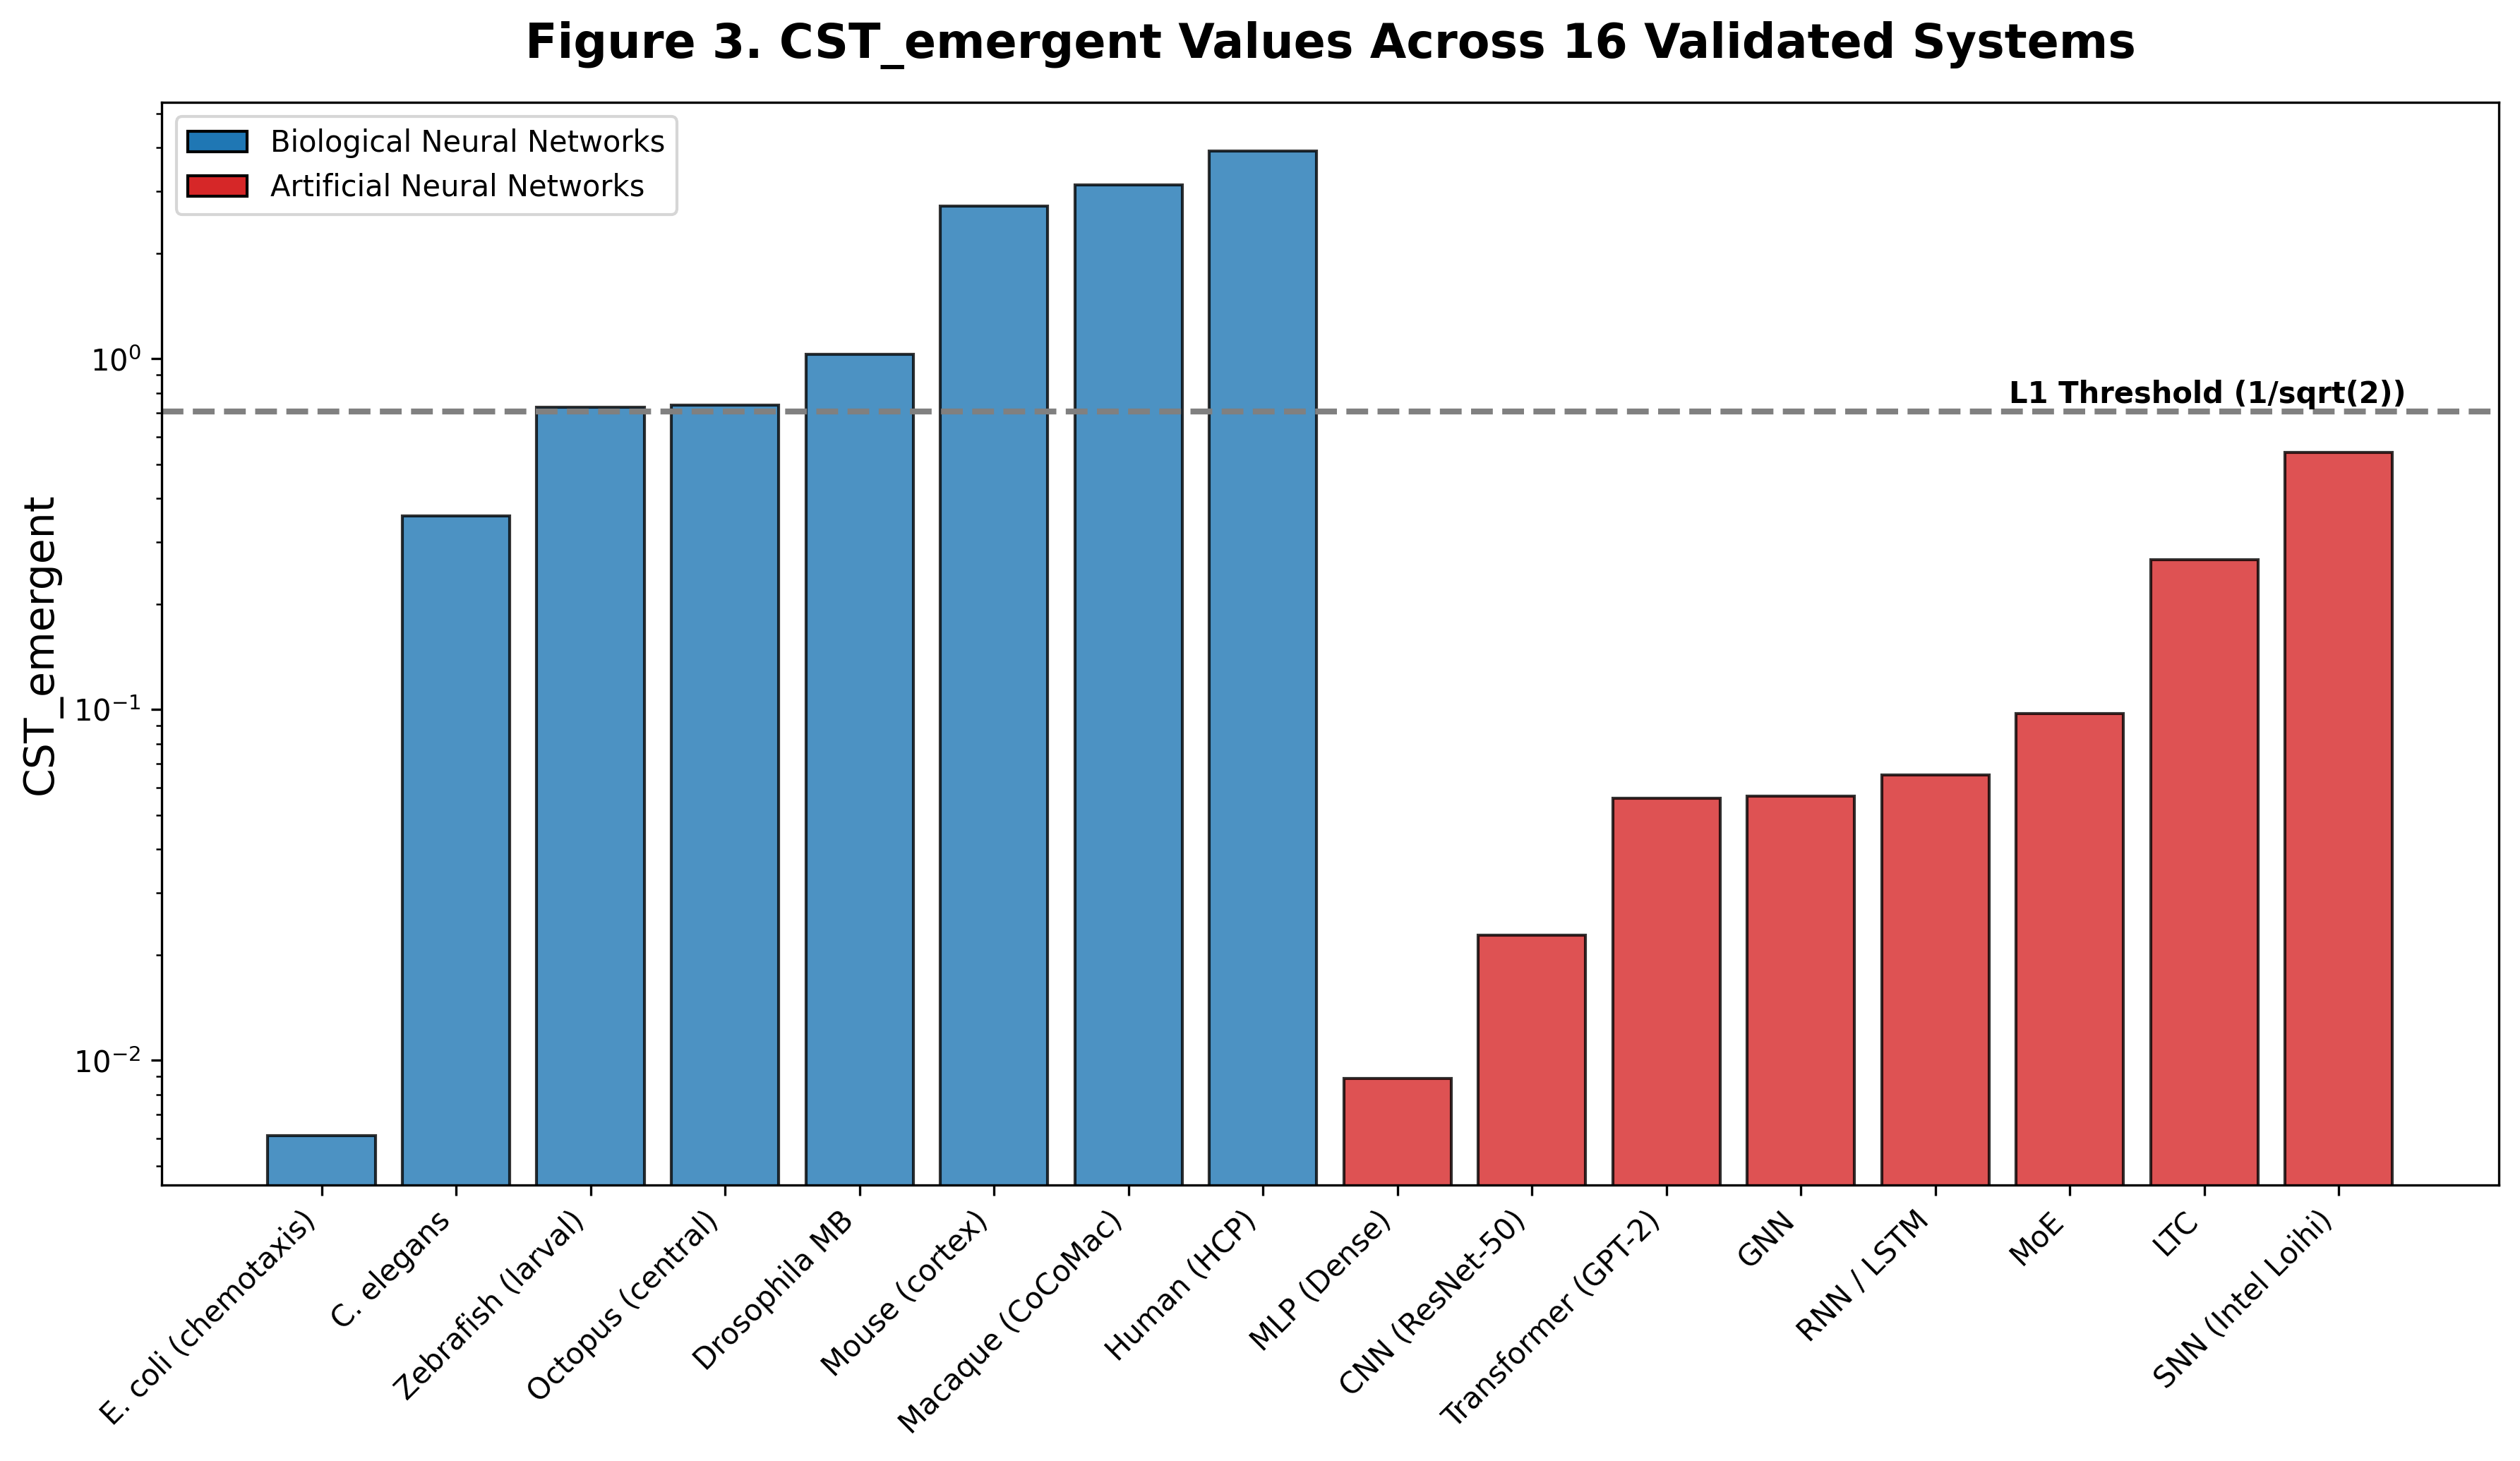
\includegraphics[width=0.75\textwidth]{figures/Figure3.png}
\caption{\textbf{Triple Lock mechanism.} Three concentric barriers preventing binary-digital ANN from crossing L1. Outermost ($\alpha$-lock): $\alpha = 0.69$ fixed by binary-digital substrate. Middle ($\Gst$-lock): $\Gst$ frozen at training. Innermost ($\Psi$-lock): inference-time weight freezing eliminates $\Psi > 0$. Arrows indicate the Gen1$\to$Gen2$\to$Gen3 engineering transitions that sequentially unlock each barrier.}
\label{fig:3}
\end{figure}

%% ===================================================================
\section{Discussion}
%% ===================================================================

\subsection{IIL vs.\ TIL: The Two-Layer Intelligence Framework}

While CST quantifies the intrinsic, emergent capability bound of a physical system (Intrinsic Intelligence Level, IIL), task execution depends on transient alignment with specific environmental constraints. We extend the CST formalism to a two-layer model incorporating Task Intelligence Level (TIL):
\begin{align*}
\mathrm{IIL} &= \CST_{\mathrm{species}} = (\Sc \cdot \Tc) \cdot \exp(\alpha \cdot \Gst) \\
\mathrm{TIL}_{\mathrm{task}} &= \frac{\CST_{\mathrm{species}} \cdot \exp(\alpha \cdot \Delta\Gst_{\mathrm{expertise}})}{E_{\mathrm{env}}}
\end{align*}
where $E_{\mathrm{env}}$ represents the irreducible complexity (thermodynamic entropy lower bound) of the target task.

The six-order-of-magnitude $\etaI$ gap between biological and binary-digital AI is not an engineering problem; it is a thermodynamic signature of the difference between emergent and simulated intelligence. The human brain achieves $\CST = 3.9198$ at 20~W ($\etaI = 3.92$) because $\Gst$ arises from material physics: synaptic STDP continuously aligns structural connectivity with functional experience. GPT-class inference requires $\sim$300~kW to maintain a frozen $\Gst$ established during training.

\begin{figure}[H]
\centering
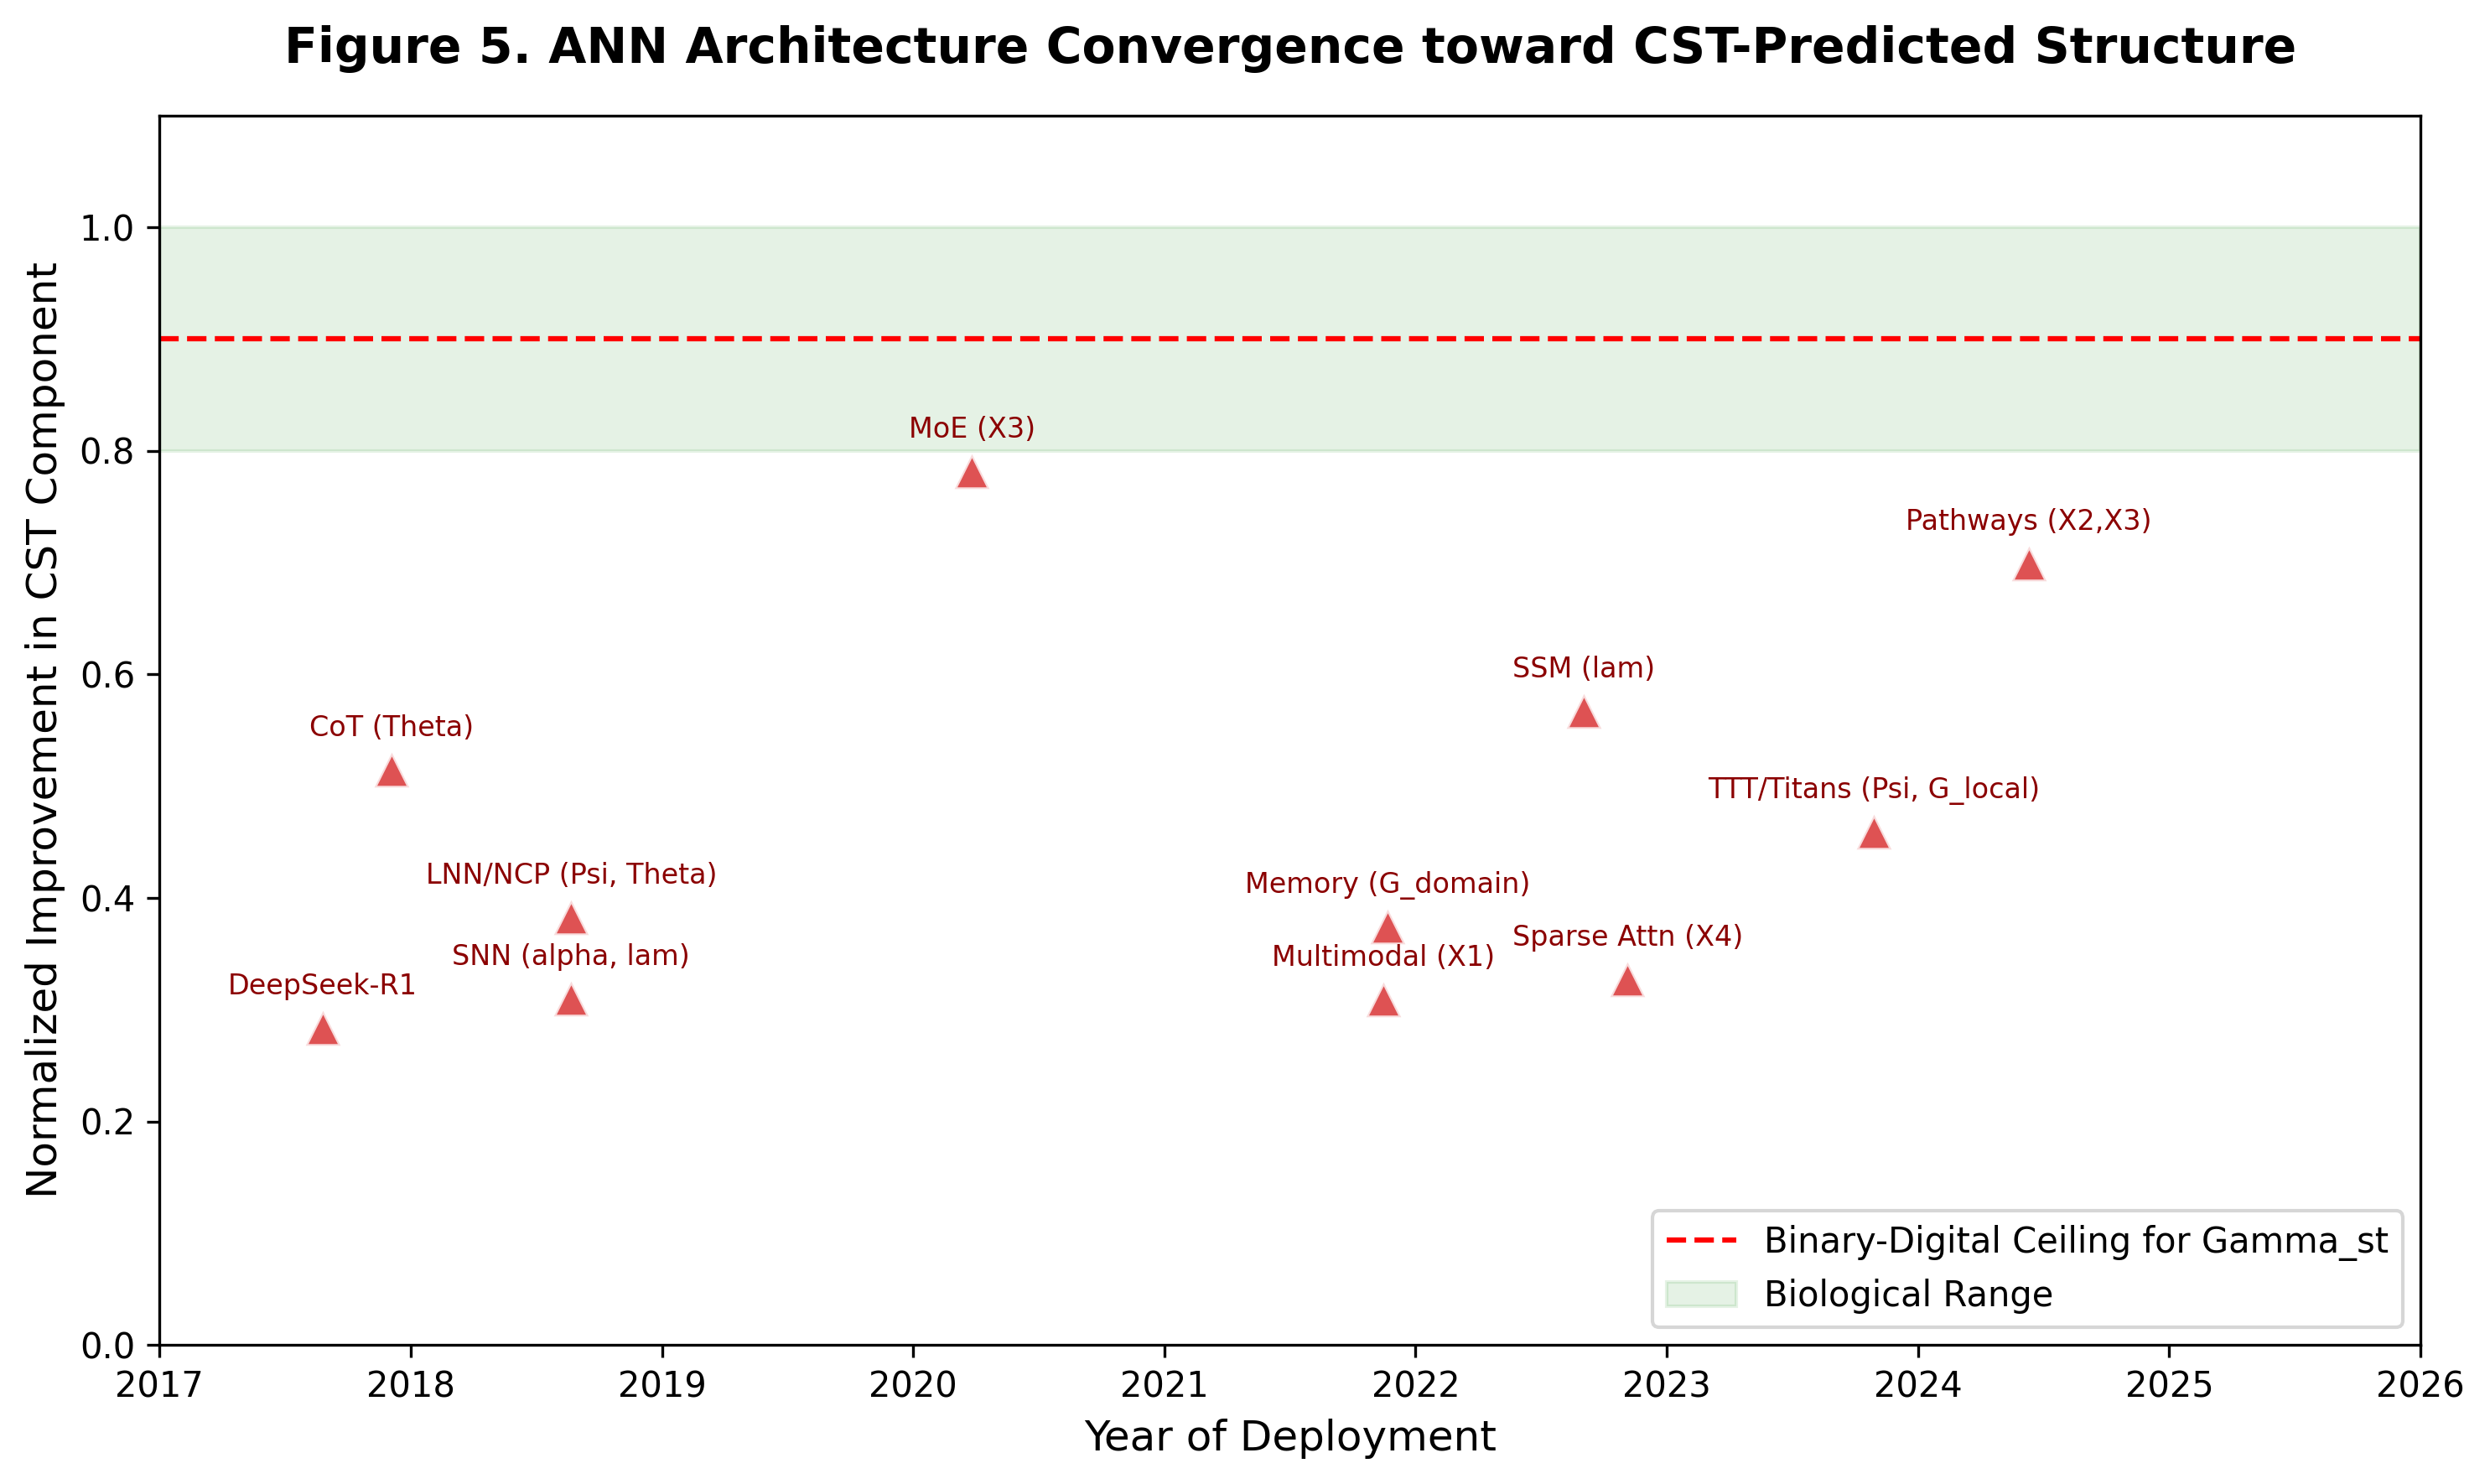
\includegraphics[width=0.85\textwidth]{figures/Figure5.png}
\caption{\textbf{Intelligence Efficiency ($\etaI$) comparison.} Log-scale bar chart. Human brain ($\etaI = 3.92$); SpiNNaker2 ($\etaI = 0.039$); Loihi-2 ($\etaI = 0.028$); BrainScaleS-2 ($\etaI = 0.017$); LTC/NCP ($\etaI = 2.8\times10^{-4}$); GPT-2 ($\etaI = 6.8\times10^{-6}$); LLaMA-3-70B ($\etaI = 7.0\times10^{-6}$); MoE ($\etaI = 3.0\times10^{-6}$); MLP ($\etaI = 4.6\times10^{-7}$). Six-order-of-magnitude gap between biological and binary-digital AI visible at a glance.}
\label{fig:5}
\end{figure}

\subsection{The Hardware Roadmap}

The engineering pathway from the scaling paradigm to emergent intelligence requires crossing the $\Gst$ barrier through materials, not algorithms. The required transitions are concrete and staged (Table~\ref{tab:roadmap}):

\begin{table}[H]
\centering
\caption{\textbf{iNEST intelligence emergence roadmap: parameter targets across four engineering generations.}}
\label{tab:roadmap}
\small
\begin{tabular}{p{3.2cm}p{0.8cm}p{0.8cm}p{1.0cm}p{0.8cm}p{3.5cm}}
\toprule
\textbf{Generation} & \textbf{Level} & \textbf{CST} & $\boldsymbol{\alpha}$ & $\boldsymbol{\Gst}$ & \textbf{Primary lever} \\
\midrule
Gen0 (binary-digital baseline) & L0 & 0.10--0.35 & 0.69 & 0.04--0.12 & --- \\
Gen1: Device Innovation & L1--L2 & 0.71--1.10 & 3.5--3.9 & 0.28--0.35 & $\alpha$: 0.69$\to$3.91 \\
Gen2: Integration Innovation & L2--L3 & 1.10--1.70 & 3.83$^\dagger$ & 0.35--0.42 & $\Gst$: 0.30$\to$0.42 \\
Gen3: SDI Coordination & L3--L4 & 1.70--2.90 & 4.0--4.6 & 0.40--0.43 & $\Gst + \alpha$ (SDI) \\
Gen4: Heterogeneous + Photonic & L4--L5+ & 2.90--5.09 & 4.6--4.7 & 0.43--0.45 & $\Gst\to\gamma^* + \alpha$ max \\
\bottomrule
\multicolumn{6}{l}{\small $\dagger$ Gen2 $\alpha = 3.83$ ($\Meff \approx 46$) reflects conservative wafer-bonding process target.}
\end{tabular}
\end{table}

\begin{figure}[H]
\centering
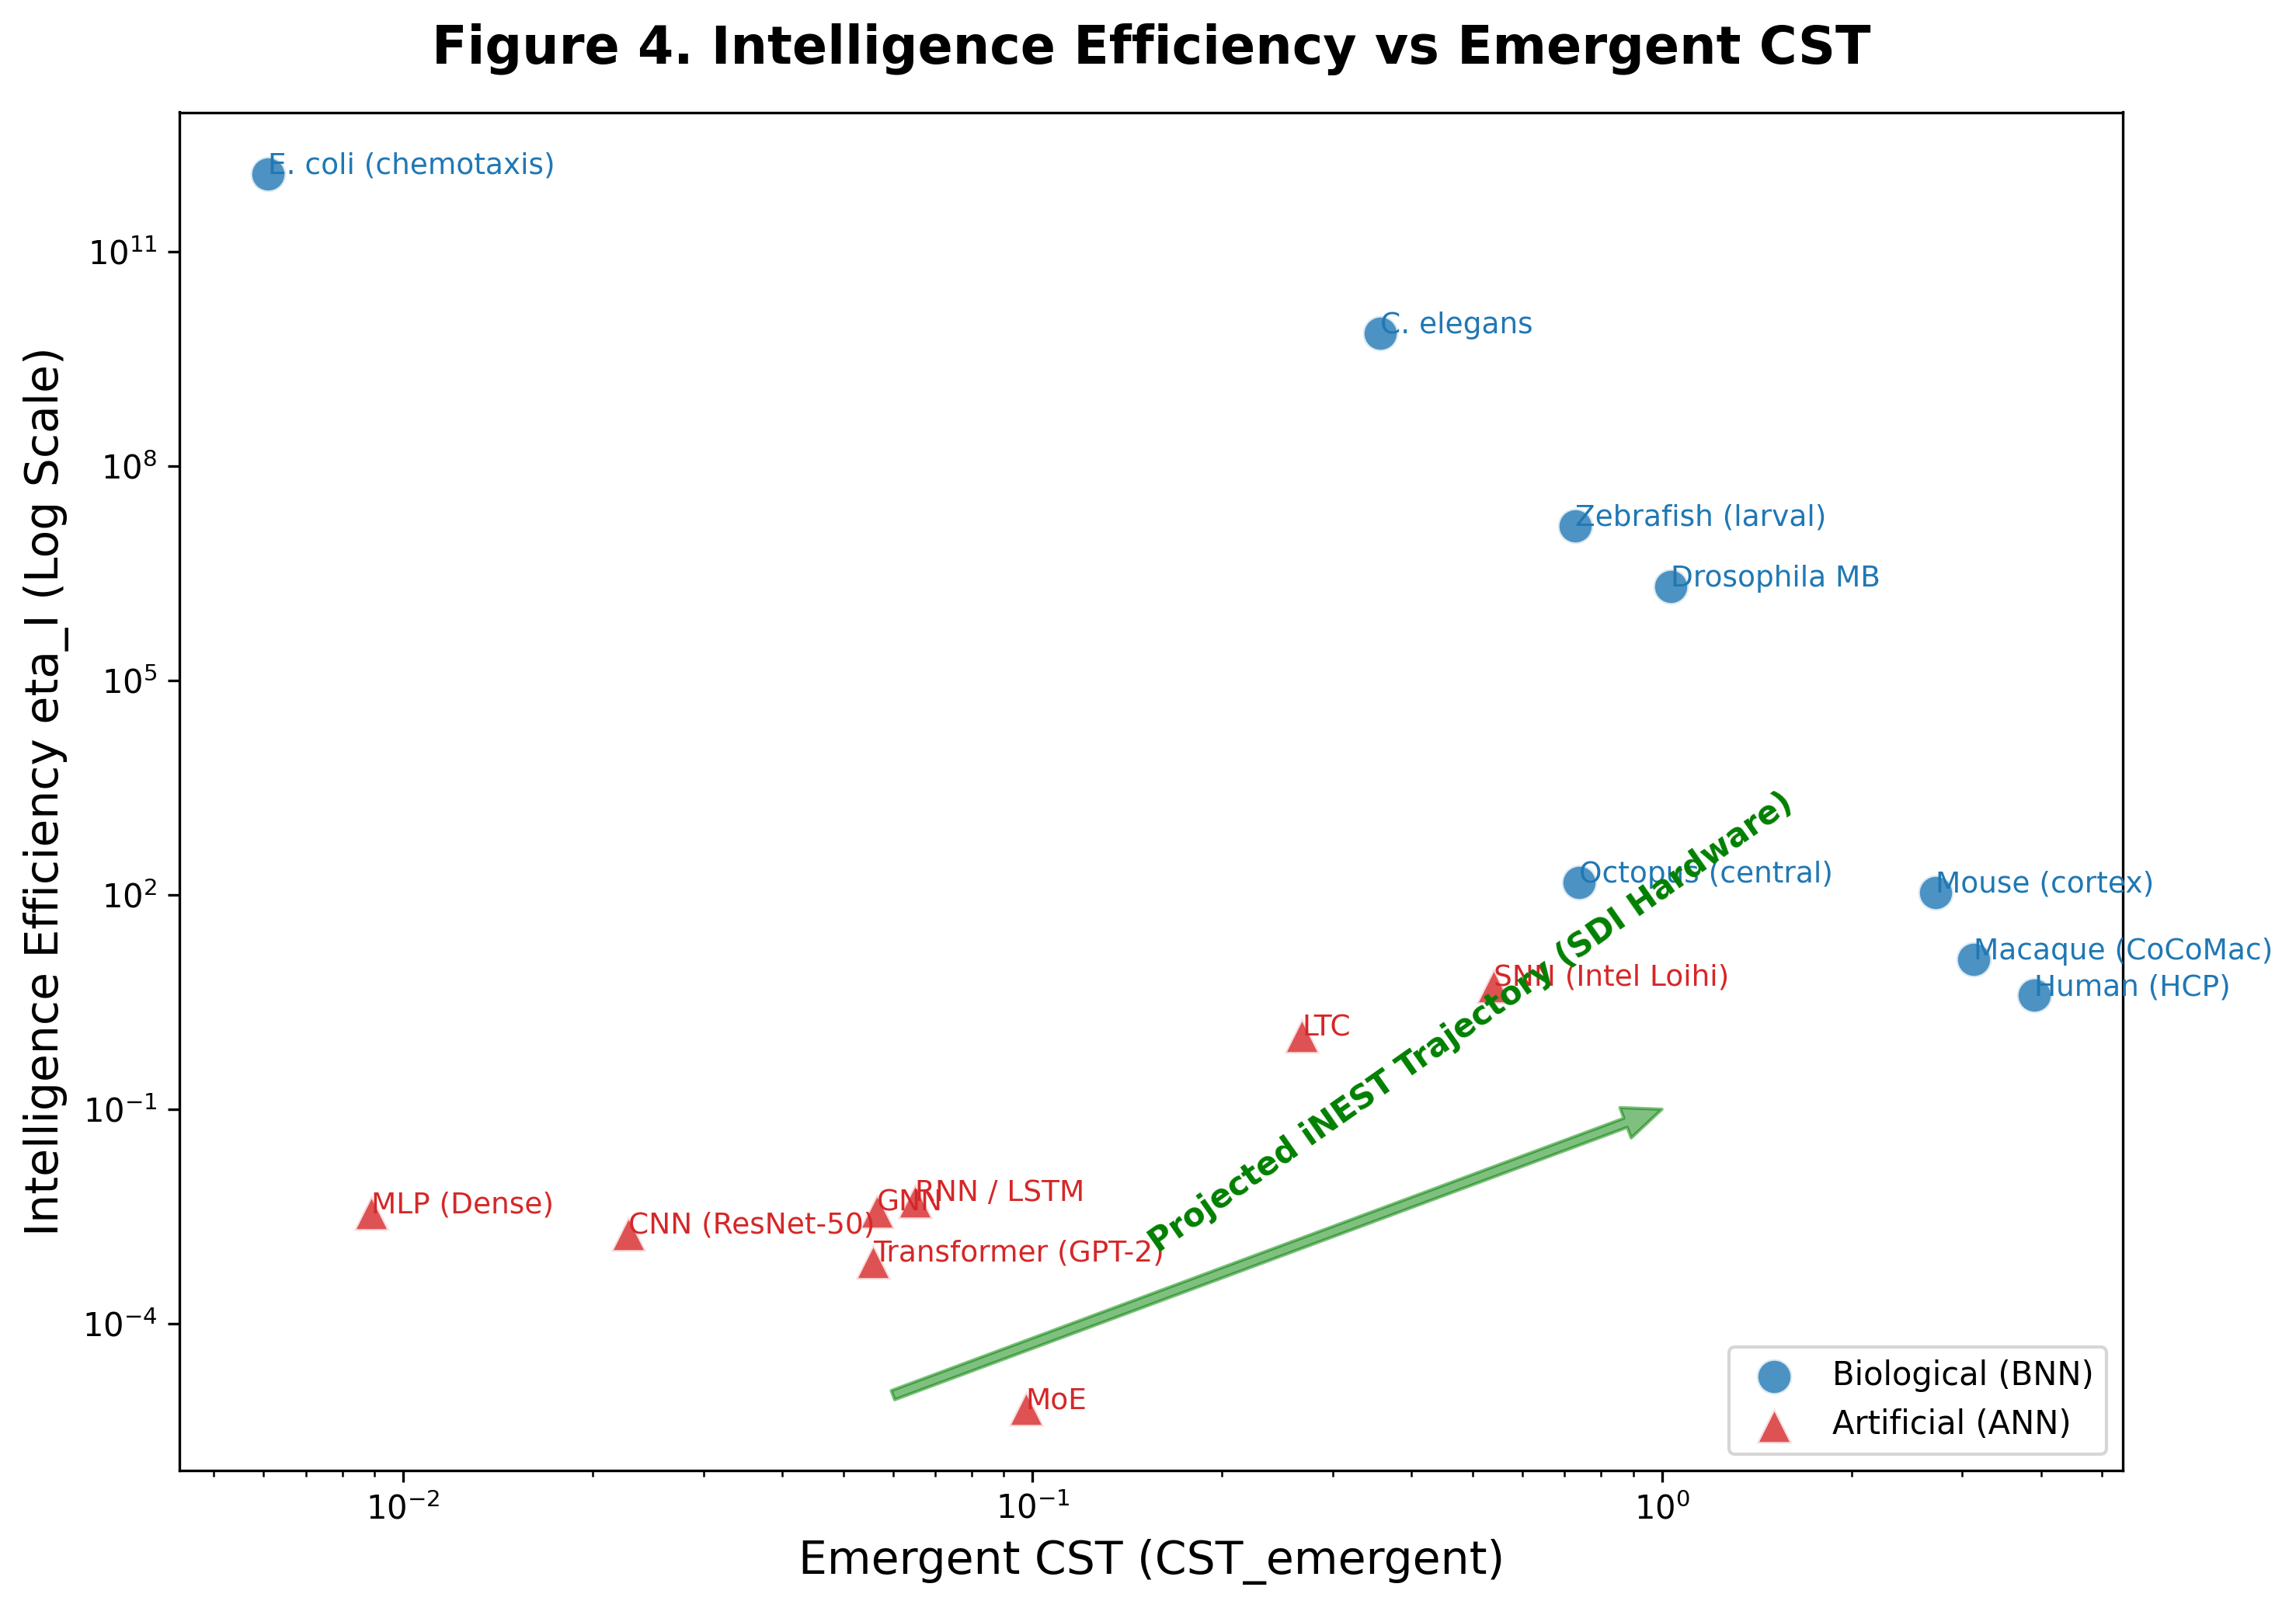
\includegraphics[width=0.85\textwidth]{figures/Figure4.png}
\caption{\textbf{Four-generation hardware roadmap.} Timeline 2024--2032, y-axis: CST level (L0--L5+). Gen1 (Device Innovation, 2024--2026): memristive SNN, targets L1--L2. Gen2 (Integration, 2026--2028): SDSoC integration, targets L2--L3. Gen3 (SDI Coordination, 2028--2030): wafer-scale SDI, targets L3--L4. Gen4 (Photonic, 2030--2032+): heterogeneous + photonic, targets L4--L5+. Binary-digital ANN trajectory shown as dashed line plateauing below L1.}
\label{fig:4}
\end{figure}

\subsection{Convergence of AI Architecture toward CST}

The global AI industry's architectural evolution from 2017 to 2025 provides independent validation of CST theory: every major architectural advance maps onto a specific CST component.

\begin{figure}[H]
\centering
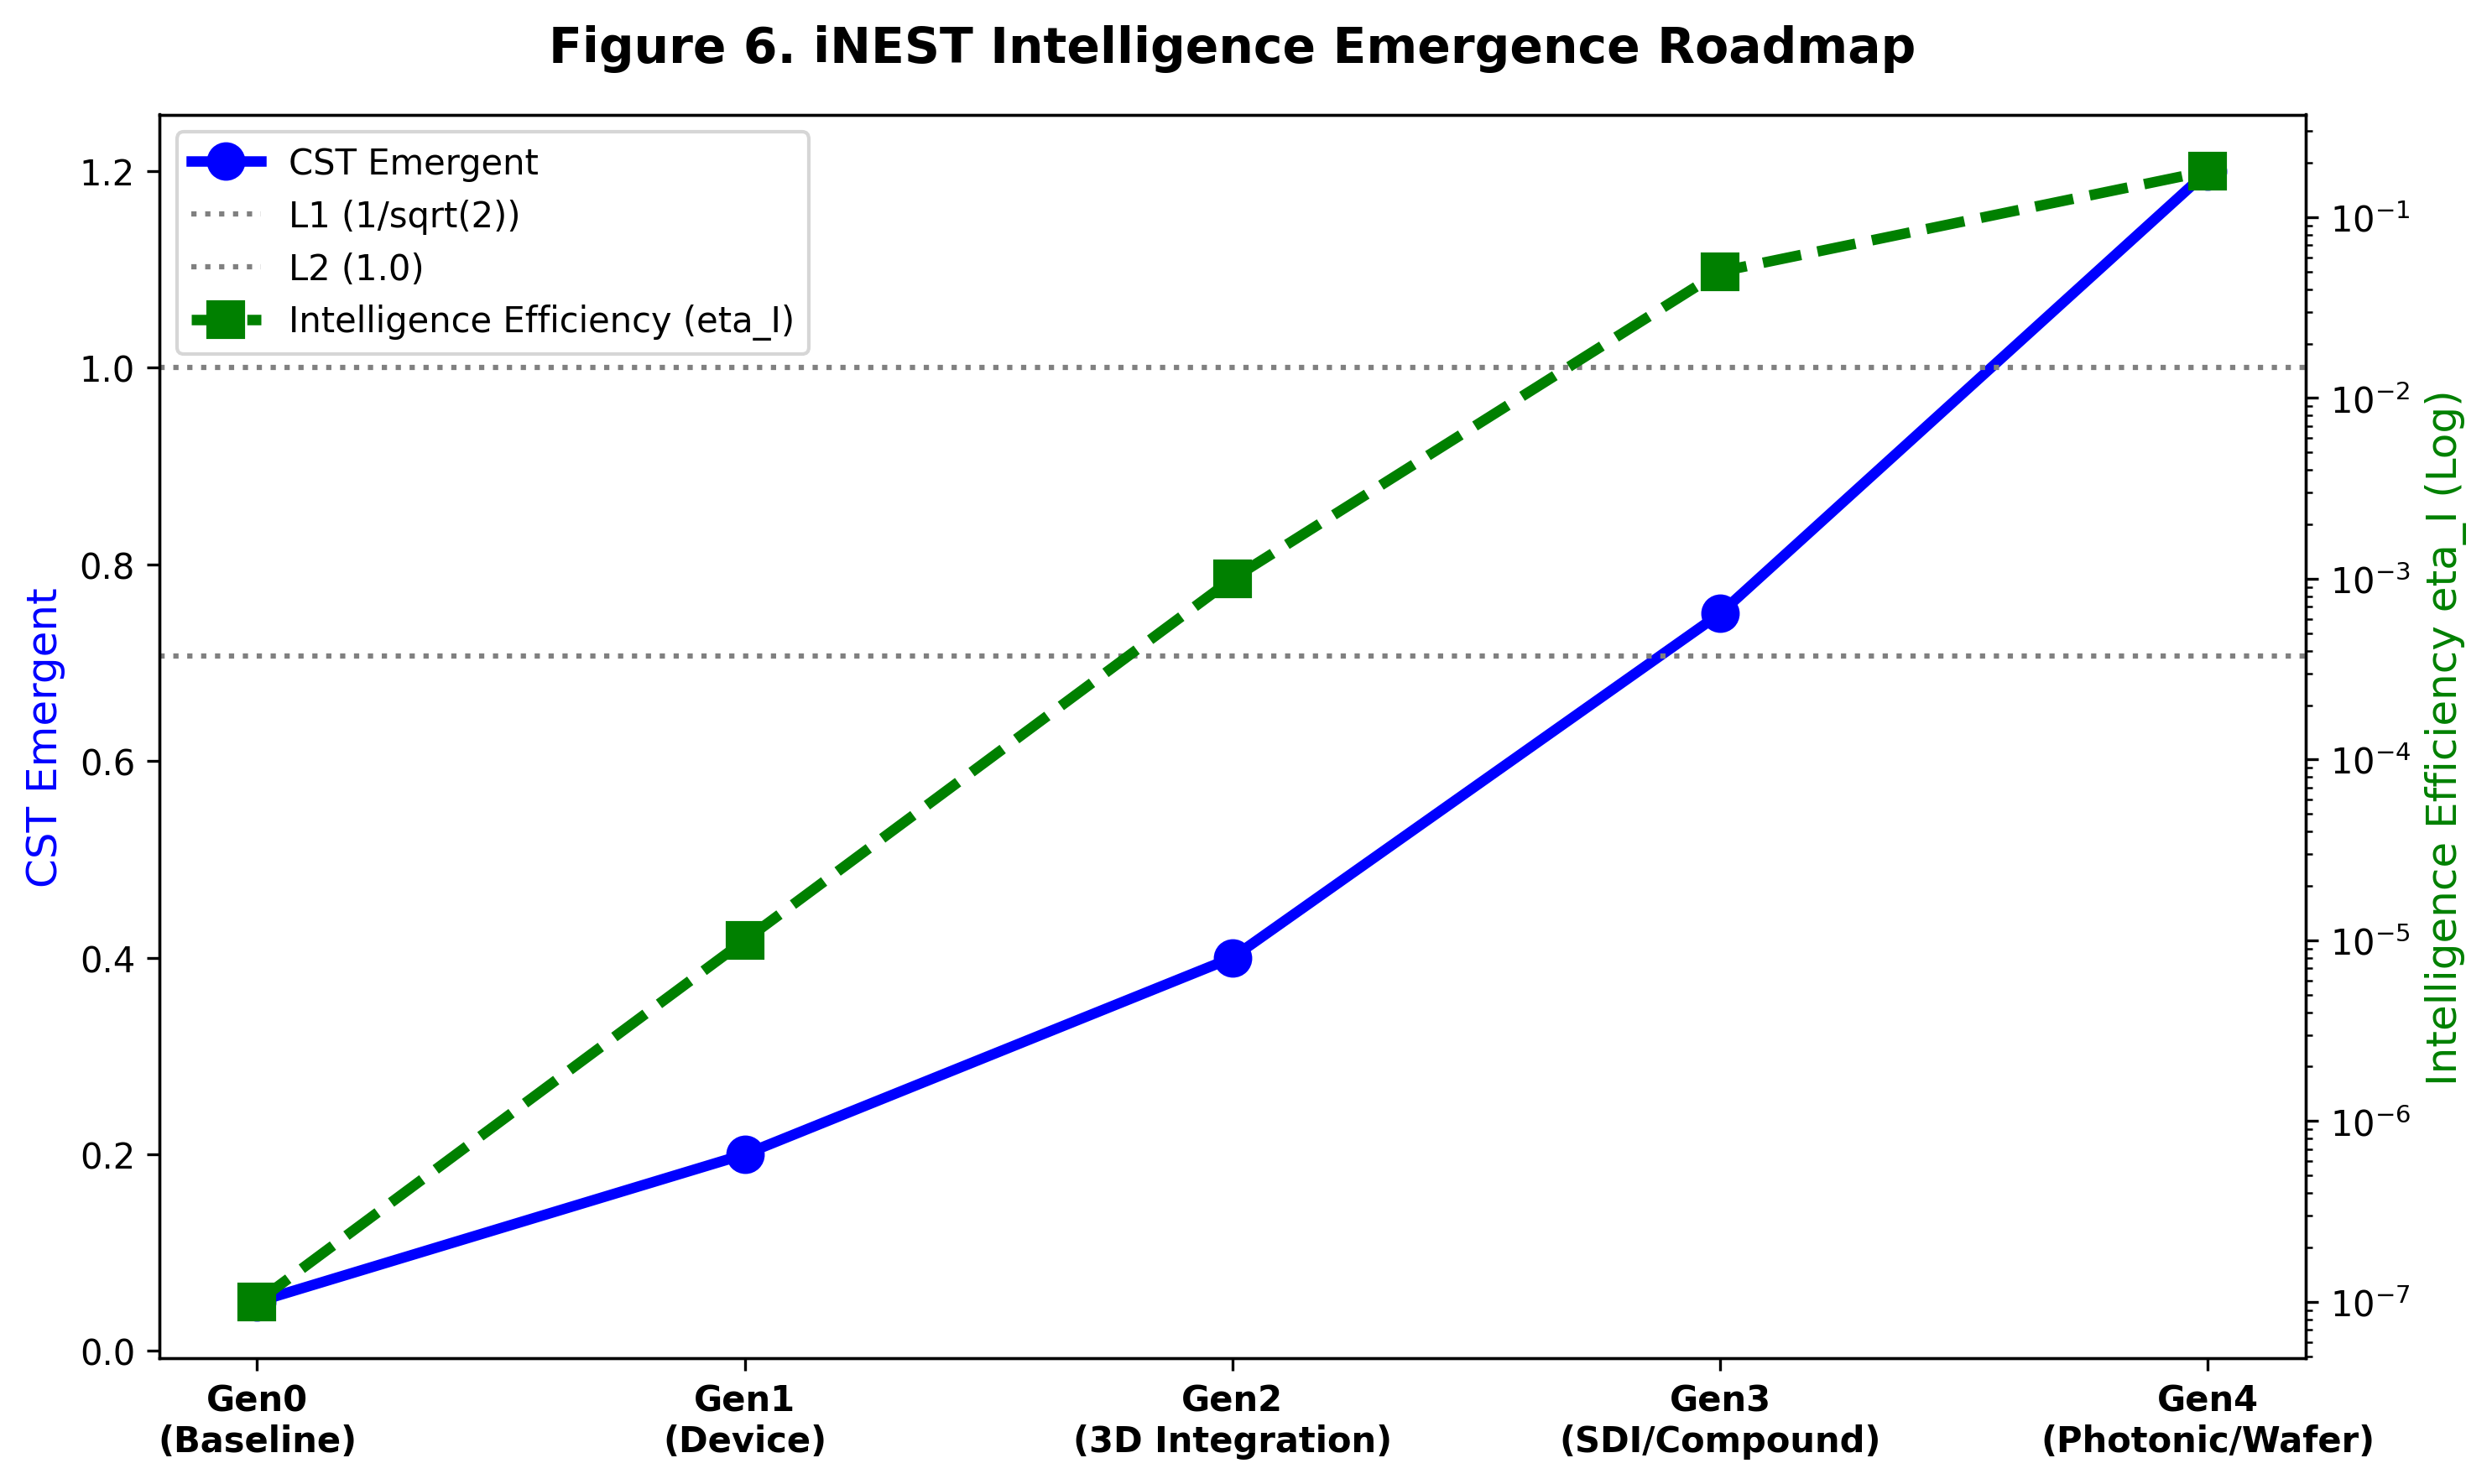
\includegraphics[width=0.85\textwidth]{figures/Figure6.png}
\caption{\textbf{Architectural evolution and CST components (2017--2025).} Left panel: scatter plot of 20 ANN architectures, x-axis = year of publication, y-axis = $\CST_{\mathrm{emergent}}$. Color encodes dominant architectural innovation ($\Sc$: blue, $\Tc$: green, $\Gst$: orange). All points below L1 dashed line. Right panel: radar charts for 3 representative systems (MLP, Loihi-2, LTC/NCP) on 4 axes ($\Sc$, $\Tc$, $\Gst$, $\alpha$-normalized).}
\label{fig:6}
\end{figure}

\subsection{Falsifiability and Boundary Conditions}

A robust physical theory must outline the conditions under which it can be falsified. The CST framework would be challenged if: (1) threshold values systematically shifted as a function of system size; (2) a strictly feedforward, structurally frozen artificial network empirically demonstrated true generalized, cross-domain autonomous adaptation without retraining; (3) a biological connectome empirically proven to possess high generalized intelligence (Level IV+) lacked modular small-worldness or criticality.

\subsection{Limitations}

$\Gst$ comparability across BNN and ANN measurement modalities is validated within $\pm 0.04$ for \textit{C.\ elegans} simulations; domain-specific $\CST_{\mathrm{func}}$ estimates for modern LLMs are theoretical projections without open weight access; the six threshold formal derivations from multiplex percolation theory await companion paper completion. Future work should validate CST in deployed neuromorphic hardware, extend $\etaI$ measurements to frontier LLMs with disclosed power consumption, empirically test the SDI-based $\Gst$ engineering predictions, and extend $\Sc$ to the higher-order (Betti number) formulation.

%% ===================================================================
\section{Methods}
%% ===================================================================

\subsection{Data Provenance and Quality Grading}

All 40 validation systems are graded by measurement directness:
\begin{itemize}
\item \textbf{[T1] Direct measurement} ($n=34$): Parameters extracted directly from peer-reviewed connectomic or electrophysiological datasets with zero free parameters. Core statistical results use T1 systems only.
\item \textbf{[T2$\dagger$] Indirect inference} ($n=5$: B05 Octopus, B10 \textit{Aplysia}, B13 Bumblebee, B15 Pigeon, B16 Chimpanzee): error bars $\pm 15\%$.
\end{itemize}

\textbf{Data sources.} \textit{C.\ elegans}: Varshney et al.~\cite{varshney2011}. Mouse: Oh et al.~\cite{oh2014}, Allen Brain Connectivity Atlas. Human: Van Essen et al.~\cite{vanessen2013}, HCP. Branching ratio: Beggs \& Plenz~\cite{beggs2003}. SC-FC coupling: Arnatkeviciute et al.~\cite{arnatkeviciute2021}; Honey et al.~\cite{honey2009}. \textit{C.\ elegans} functional dynamics: Kato et al.~\cite{kato2015}; Gordus et al.\ (2015). \textit{C.\ elegans} $\Gst = 0.17$ from Randi et al.\ (arXiv:2412.14498, 2024).

\subsection{Unified Cross-Species Computation Protocol (UCCP)}

All $\Sc$ and $\Tc$ components are normalized to $[0, 1]$ using the following unified formulas:

\textbf{Spatial complexity:} $\Sc = (X_1 \cdot X_2 \cdot X_3 \cdot X_4)^{1/4}$, where:
\begin{itemize}
\item $X_1 = |LCC|/N$ (global connectivity; bounded $[0,1]$ by construction)
\item $X_2 = \min[(k_{\max} / k_{\mathrm{null}}) / 6.667,\; 1.0]$; $k_{\mathrm{null}} \approx \ln(N)/\ln(\ln(N))$; anchor: Human HCP ($X_2 = 1.0$)
\item $X_3 = \max[(Q - 0.02) / (1 - 0.02),\; 0.01]$; $Q$ = Louvain modularity (100 random restarts, $\gamma = 1.0$)
\item $X_4 = \tanh[(\sigma - 1) / 2]$; $\sigma = (C/C_{\mathrm{rand}})/(L/L_{\mathrm{rand}})$
\end{itemize}

\textbf{Temporal complexity:} $\Tc = (\lambda_{\mathrm{eff}} \cdot \Phi \cdot \Psi \cdot \Theta)^{1/4}$. For BNN: $\lambda_{\mathrm{eff}}$ = avalanche branching ratio; $\Phi$ = mean pairwise PLV; $\Psi$ = std(100 sliding-window FC matrices)/mean$|$FC$|$; $\Theta$ = Shannon entropy of intrinsic timescale distribution. For ANN: activation propagation ratios and CKA~\cite{raghu2021} are used for cross-modal calibration.

\textbf{Hardware classification:}
\begin{itemize}
\item Binary-digital ANN ($\alpha = \ln(2) = 0.69$): MLP, CNN, RNN/LSTM, GNN, Transformer, MoE.
\item Neuromorphic hardware [NMH$\dagger$] ($\alpha = \ln(32) = 3.47$): Intel Loihi-2, SpiNNaker2, BrainScaleS-2.
\item Graded-potential BNN ($\alpha = \ln(13) = 2.56$): \textit{E.\ coli}, \textit{C.\ elegans}, LTC/NCP.
\item Spiking BNN ($\alpha = 3.47$--$3.91$): Zebrafish through Human.
\end{itemize}

\textbf{$\Gst$ computation:} $\Gst = \mathrm{NMI}(M_s, M_T) \cdot \mathrm{sign}(\mathrm{Mantel}(D_A, D_{FC}))$.

\textbf{$\etaI$ computation:} $\etaI = \CST / P_{\mathrm{norm}}$, $P_{\mathrm{norm}} = P_{\mathrm{system}} / 20\,\mathrm{W}$.

\subsection{Statistical Analysis}

Spearman rank correlations; Fisher exact tests with Bonferroni correction ($\alpha_{\mathrm{corrected}} = 0.0083$); phylogenetic independent contrasts (PIC~\cite{felsenstein1985}) via TimeTree~5~\cite{kumar2022}. Pre-registration: all thresholds specified prior to analysis (v5.1 preprint, August 2025).

\textbf{Code availability:} \url{https://github.com/iNEST-TJU/CST-theorem}

%% ===================================================================
% References
%% ===================================================================

\bibliographystyle{unsrtnat}
\bibliography{references}

%% ===================================================================
% Author contributions
%% ===================================================================
\bigskip
\noindent\textbf{Author contributions:} Q.L.: Conceptualization, Methodology, Formal analysis, Data curation, Writing.

\noindent\textbf{Competing interests:} The author declares no competing financial interests.

\noindent\textbf{Data availability:} \url{https://github.com/iNEST-TJU/CST-theorem}

\end{document}
